\documentclass[a4paper, 12pt]{book}

\usepackage{natbib}
\usepackage{amsmath}
\usepackage{amssymb}
\usepackage{amsfonts}
\usepackage{graphicx}
\usepackage{adjustbox}
\usepackage[table]{xcolor}
\usepackage[toc, page]{appendix}

% Drawing
\usepackage{tikz}
\usetikzlibrary{matrix}
\usetikzlibrary{shapes,arrows}

% Expectation symbol
\DeclareMathOperator*{\E}{\mathbb{E}}

% Cool titles
\usepackage{sectsty}
\allsectionsfont{\sffamily}

\begin{document}
\tableofcontents

\newpage

% Introduction 
\chapter{Introduction}

This paper presents an algorithm for surface classification using millimeter-wave radar. 

Fundamentally, radar is based on the concept of transmitting and recieving electromagnetic radiation. Radar response depends on the surrounding region of the sensor as objects in its vicinity scatter transmitted waves differently \citep{richards_2014}.  

 As technolgy is becoming increasingly intertwined with everyday life a multitude of new areas for smart sensing has opened up. One sensor category that has been recieving much attention is radars with very high frequency. These sensors combine a multitude of desirable features packed into a favorable form factor. These capabilities has made high frequency radars an increasingly popular choice in a steadily growing number of applications, such as monitoring of vital signs \citep{kuo_lin_yu_lo_lyu_chou_chuang_2016}, gesture recognition \citep{lien_gillian_karagozler_amihood_schwesig_olson_raja_poupyrev_2016}

Alongside with this development another trend within data science has emerged; the movement towards machine learning centric methods . This transition, spanned over multiple decades, has placed machine learning as one of the main-stays of information technology and a rather central part of our life. With ever increasing amounts of data, smart data analysis has proven key for technological progress \citep{a_smola_svn_vishwanathan_2010}.

Machine learning algorithms fundamentally utilizes various statistical techniques in order to allow computer systems to progressively improve performance. Data scientists have found this subclass of aritficial intelligence extremely practical, especially for data that lack an easily predictable structure. 

The amount of millimetre-wave radar applications is growing steadily.

With a continuously increasing demand for small sensors for use in a world where 

\section{Motivation}

Classification of surfaces is an important task which appears in many areas. There are already numerous methods for classifying surfaces based on, for instance, optics and probing. For example, using images have been a successful approach in determining surface roughness. One such method involves images of three-dimensional surface textures under different directions of illumination, and after some image processing techniques using a support vector machine for classification \citep{dong_duan_yang_2008}. 

For probing on the other hand one resorts to measuring directly onto a surface. By sweeping a thin film across a fabric with constant contact force a depth-dependant charge is induced. After reading the output charge over some time interval it is then possible to extract information for detecting the texture of the fabric \citep{song_han_hu_li_2014}. A similar approach was used in \citep{strese_schuwerk_iepure_steinbach_2017}, where again surface classification was performed through direct contact. In this case features where instead extracted from the sound produced by vibrations generated by the movement. 

Both of the approaches above have drawbacks. 

optical, probing etc.
\\ \\
\noindent Optical: Images has been successful in determining surface roughness. One such method involves images of three-dimensional surface textures under different directions of illumination, and after some image processing techniques using a support vector machine for classification \citep{dong_duan_yang_2008}. 
\\ \\
\noindent Probing: One may also measure directly onto a surface directly through a probing approach. By sweeping a thin film across a fabric with constant contact force a depth-dependant charge is induced. After reading the output charge over some time interval it is then possible to extract information for detecting the texture of the fabric \citep{song_han_hu_li_2014}. A similar approach was used in \citep{strese_schuwerk_iepure_steinbach_2017}, where again surface classification was performed through direct contact. In this case features where instead extracted from the sound produced by vibrations generated by the movement. 
\\ \\
It is often desirable to to this without direct contact i.e. probing
\\ \\
Localization is the classic use-case for radars. 
\\ \\
 Radar  can detect relatively small targets at near or far distances and can measure their range with  precision  in  all weather,  which is  its chief  advantage when compared with other  sensors \citep{skolnik}
\\ \\
Radar classification: Previous work and how they are different: A major challenge in radar sensing is to not only detect, but also to identify radar targets. This can for example be used for monitoring of urban environments \citep{harter_kowalewski_sit_jalilvand_ziroff_zwick_2014}, or with a radar system mounted on a rotary table unit. 

 of urban environments and automotive radar 
\\ \\
Applications involving millimetre-wave radars and surface recognition is scarce.  
\\ \\
These radars commonly have wavelenghts of something something
\\ \\
If we however want to classify surface materials using a much shorter wavelength, the task changes dramatically as apsorption is near-instant. 
\\ \\
Something about radar wavelenght categories
\\ \\
Furthermore, radar sensors are commonly used in an array setting which permits beamforming and extraction of spatial information. 
\\ \\
If one on the other hand only has a singular radar sensor this is not possible and you must resort to other means.
\\ \\
Probably want something about IQ demodulation somewhere in here.

\section{Problem formulation}
With this work, we intend to present a solution towards surface identification based on radar data. The data is collected using two 60 GHz Acconeer radar sensors, each with a sampling frequency of 200 Hz. Both sensors are mounted at the front of a robot, and are assumed to move across a surface with a constant speed and height.

Once obtained, the data will undergo feature extraction. Ideally, we want few features that carry as much information as possible. The next step is to develop a machine learning model into which these features will be feeded. Several different model types will be investigated and evaluated, after which we choose one to proceed with and optimize. 

The working procedure is illustrated in figure (....)

%We develop a pipeline for effectively solving this problem. 
%\\ \\
%We present modelling options with high accuracy and efficacy. 
%\\ \\ 
%We present results based on a 60GHz Acconeer micro radar. 
%\\ \\
%In this paper we introduce means of surface identification based on the output from a single 60 GHz radar sensor moving across a surface with constant height. 

\section{Thesis outline}

In chapter 2 we present an overview of a general radar system and introduce some crucial concepts for understanding the radar output used in this work. In chapter 3 we proceed by presenting our measurement setup and comment on the data collecting process and the data itself. Chapter 4 revolves around discussing ways of preprocessing the data and extracting relevant features from it. After the preprocessing, in chapter 5, we go through different classification schemes we have tested. The classification results are presented in a table for easy comparison. Finally, we conclude with an overall discussion of the work in chapter 6 and summarize our conclusions in chapter 7.

%Chapter 3: Mention something about the data collecting process. Motive our choice of parameters such as sampling frequency. Go through visual observations of our data.

%Chapter 4: Feature selection and preprocessing is considered. Signal structure is discussed primarily on an intuitive level. 

%Chapter 5: Classification schemes. Moving from simple to advanced, some classifiers of special interest are investigated. Results with regards to these classifiers are presented.

%Chapter 6: Disucssion.

%Chapter 7: Conclusion.


% Radar system overview
\chapter{Radar System Overview}

In order to build a model capable of accurately capturing key features from target surfaces one must first understand the origin of the received signal. In this chapter a few fundamental concepts in radar systems are introduced that explain how range, velocity and reflectivity arise in a \gls{pcr} system. The mixing and \gls{iq} demodulation procedures are also discussed, which explain how a returning radar echo is captured and demodulated. 

\section{Target Properties from Radar Response}
% TODO: Utilize https://acconeer.sharepoint.com/:w:/g/CS/ES_xwcoTqVdGkShPJkNagMMBL1wVd_GaeJJsEDKC8lWIDQ?e=GxZNEw as a source for this.
Fundamentally, a radar operates by radiating \gls{rf} electromagnetic energy and listening if the transmitted energy generates any echoes \citep{skolnik_2009}. By analyzing properties of returning signals it is then possible to obtain information regarding the scattering targets. This may involve the distance and angle at which scatterers are located or at which velocity they are moving in. With a sufficiently high angular and range resolution it is even possible to discern parts of the targets' shapes and sizes.  

Standard radars are active systems, meaning that they have a radiating antenna and hence do not depend on any ambient radiation for target identification \citep{richards_2014}. Radar systems can be realized in many ways, however in this report a \gls{pcr} system is used. This means that a sequence of short coherent wavelets are transmitted towards a target scene to determine its properties. One such transmitted wavelet pulse $x_T(t)$ has some carrier frequency $f_c$ and envelope $A(t)$ as in

\begin{equation}\label{eq:trans}
	x_T(t)
	= A(t)\sin(2\pi f_c t).
\end{equation}

After various scattering processes, the returning signal is captured by either an array of antennas, or just a single antenna.

\subsection{Single-Antenna Considerations}

Commonly, in larger radar systems, many receiving antennas capture the returning radiation. This allows for distinguishing radar targets not only in range, but also in angle. In this work a single receiving antenna is used, meaning that the radar has no intrinsic method of determining at which angle a scatterer is located. Thus, only range information can be captured by this sensor. 

To understand what information can be obtained from such a one dimensional signal, a single scattering object some distance away from the transmitter is here considered. If a radar pulse with envelope $A(t)$ and frequency $f_c$ is transmitted towards it, the returning signal will be a delayed pulse on the form \citep{richards_2014}

\begin{equation}\label{eq:returning}
	y(t) = CA(t-B)\sin(2\pi f_t (t-B))
\end{equation}
where $B$ is some delay related to the distance to the target and $C$ a constant correspoding to the loss of energy from transmission to reception of a pulse. For the purposes of this report, the properties of this delay is of particular interest. In the next two sections, it is shown how distance and velocity can be deduced from this parameter using absolute measurements of $D$ and relative changes in $D$ between pulse measurements. The $C$ variable carries information about the reflectivity of a scatterer, described lastly. 

\subsection{Radar Distance Measurements}

If a point scatterer was present a distance $d$ from the transmitting antenna, a wavelet will return $2d/c$ seconds after transmission, where $c$ denotes the speed of light. The 2 appears to accomodate for the pulse traveling back and forth (or, perhaps more accurately, forth and back) between the sensor and the scatterer. Hence, the transmitted signal is delayed according to 

\begin{equation}
	\begin{split}
		y(t) 
		& = CA(t-2d/c)\sin(2\pi f_c(t - \frac{2d}{c})) \\
		& = CA(t-2d/c)\sin(2\pi f_ct - \frac{4\pi d}{c}f_c).
	\end{split}
\end{equation}

By measuring the delay $D$ in \ref{eq:returning} we can thus simply calculate the distance through

\begin{equation}
	d = \frac{Dc}{2}.
\end{equation}

Thus, by examining the time delay of the returning signal, we can deduce the distance to the scattering object. 

\subsection{Doppler Frequency in Pulsed Radar}\label{sec:doppler}
\label{doppler}

If the target scatterer is moving from or towards the transmitting antenna, a frequency shift will occurr. For velocity $v$, the transmitted frequency $f_c$ will be shifted to $f_r$ according to the well known Doppler formula \citep{ridenour_1947}

\begin{equation}
	f_r = \frac{c + v}{c - v}f_c
\end{equation}
where positive $v$ indicates that the scatterer is moving towards the transmitter. The frequency shift $f_d$, also known as the \emph{beat frequency} \gls{bf}, is then

\begin{equation}\label{eq:dshift}
	f_d 
	= f_r - f_c 
	= \frac{2v}{c-v}f_c \approx \frac{2v}{c}f_c 
	= \frac{2v}{\lambda_c}
\end{equation}
where $\lambda_c$ is the carrier wavelength. This shift means that the an approaching target has slightly increased returning frequency, and conversely that a receeding target has a slightly decreased frequency. In this project a pulsed radar is used, meaning that measurements are done repeatedly using short wavelets instead of transmitting one continuous wave. What does this mean for the Doppler shift?

For a pulsed coherent radar system, with sampling frequency $F_s$ and sampling period $T_s = 1/F_s$, the Doppler shift can instead of a shift in frequency be viewed as a phase shift from one pulse to the next. Between two pulses, a target moves a distance $vT_s$. Hence, each pulse travels a distance $2vT_s$ less than the preceding one. This distance corresponds to $2vT_s/\lambda_c$ wavelengths, providing a phase change $\Delta \phi$ per pulse of

\begin{equation}
	\Delta \phi = \frac{4\pi}{\lambda_c}vT_s.
\end{equation}

For a target moving at a constant pace, the \gls{bf} arising from the constant doppler phase shift is thus $f_d = 2v/\lambda_c$, as was found in equation \ref{eq:dshift}. Thus, by taking a discrete fourier transform (\gls{dft}) of the sequence of $T_s$-spaced measurements for one specific distance, we can estimate the velocity from the peak frequency $f$ in this signal as 

\begin{equation}\label{eq:dopp}
	v = \frac{\lambda_c f_d}{2}
	\approx \frac{\lambda_c f}{2}.
\end{equation}


\subsection{Power Dissapation}

The $C$ factor in \ref{eq:returning} describes the ratio of the emitted power that is received after a scattering process has occurred. To get a feel for how a targets' reflectivity relates to this factor we can make the following thought experiment. First we assume that the trasmitted power $P_t$ is radiated isotropically by a point source, meaning that the power density is distributed uniformly by the source over the surface of a sphere. When our radar "balloon" has radius $R$, the power density at the balloon surface becomes  \citep{amin_2017}

\begin{equation}
	P_d 
	= \frac{P_t}{4\pi R^2}.
\end{equation}

If a scatterer is present at range $d$ with radar cross section (\gls{rcs}) $\sigma$ and gain $G_t$, the fraction of the radar power reflected by the scatterer is given by 

\begin{equation}
	P_{e}
	= \frac{P_tG_t\sigma}{4\pi d^2}.
\end{equation}

Then, given that the scattering process also is isotropic, the power reflected back at the radar receiver is

\begin{equation}\label{eq:temp}
	P_f 
	= \frac{P_e}{4\pi R^2} 
	= \frac{P_t G_t \sigma}{(4\pi d^2)^2}.
\end{equation}

Finally only a portion $P_r = P_fA_r$ of the power is captured by the receiver, where $A_r$ is a function of transmission wavelength and receive antenna gain. Including this into \ref{eq:temp}, we obtain the \emph{radar range equation} (\gls{rre}) relating the transmitted and recieved power as

\begin{equation}
	P_r
	= \frac{P_t G_t A_r \sigma}{16\pi^2 d^4}.
\end{equation}

The radar range equation states that power dissapates rapidly, by a factor $1/d^4$, with range. Hence, increasing the distance to a target object by a factor 2 will return only $1/16$ of the power otherwise received. According to \citep{richards_2014} this rate is in real-world scenarios typically between $1/d$ to $1/d^4$, so that the process may not be as lossy as the \gls{rre} predicts. If the noise power $N$ remains constant regardless of target distance, the \emph{signal-to-noise ratio} (\gls{snr}), defined as $\text{SNR} = P_r/N$ quickly decreases with range\footnote{Note that this argument only holds for scatterers of limited size, and that if the scattering target for instance was a parabolic antenna, a waveguide or a large wall this relationship between the transmitted and received power would not be valid.}. 

We also see from the \gls{rre} that the power returned is governed by the \gls{rcs} $\sigma$ of the target. The \gls{rcs} describes how reflective a target is, determined both by its size as well as its dielectric properties. It can be regarded as a fictious area that describes the intensity of the wave reflected back to a scatterer. This area is the projected area of an electrically large, perfectly conducting sphere whose echo strength would match that of the target if we were to replace the target with the sphere \citep{knott_1993}. 

However, as the reflectivity and thus the \gls{rcs} can vary with both distance and viewing angle, this fictious metal sphere subsequently changes size depending on where in space it is located. Thus, our best recourse is to simply regard the \gls{rcs} as a measure of the intensity of the radar echo expressed in terms of an area. 

% Have a part on bandwidth
\section{Analog Convolution}

In the preceding section it was shown that the scattering response carry information about target range, reflectivity and radial velocity. This section explains how the radar captures the returning signals to generate raw radar data through \emph{analog convolution}.

Analog convolution means convolving the returning signal with the transmitted. It involves generating an internal pulse, called an analysis pulse, as a delayed copy of the transmitted pulse. The received signal and the generated signal are then multiplied elementwise and summed, to form one measurement point $m(\tau)$, where $\tau$ is the internal delay of the analysis pulse. 

Mathematically we can describe this convolution as

\begin{equation}
	m(\tau) 
	= x_T(-t) * y(t)
	= \int_{-\infty}^{+\infty} x_T(t - \tau)y(t) dt
\end{equation}
where $x_T(t)$ is the analysis pulse as defined in \ref{eq:trans} and $y(t)$ is the returing wavelet. If the incoming signal $y(t)$ stems from a single scattering point target then $y(t)$ is on the form of \ref{eq:returning}. With the envelope $A(t)$ as a rectangular envelope\footnote{The rectangular envelope is commonly used for maximal power transmission \citep{richards_2014}, however the Acconeer radar system employs an envelope more similar to a raised cosine. The rectangular envelope is used here mainly for mathematical convenience.} of length $L$

\begin{equation}
	A(t) = \begin{cases}
		1 & \text{if $0\leq t < L$} \\
		0 & \text{otherwise},
	\end{cases}
\end{equation}
$m(\tau)$ will be on the form 

\begin{equation}\label{eq:n0}
	m(\tau) = 
	\begin{cases}
		0 & \text{if $|\tau-2d/c|\geq L$} \\
		\text{(\ref{eq:n1})} & \text{if $|\tau-2d/c|<L$ and $\tau \leq 2d/c$} \\
		\text{(\ref{eq:n2})} & \text{if $|\tau-2d/c|<L$ and $\tau > 2d/c$}
	\end{cases}
\end{equation}

\begin{equation}\label{eq:n1}
	\frac{C}{2}\Big((\tau + L - B)\cos(2\pi f_c(\tau - B)) 
	- \frac{1}{2\pi f_c}\sin(2\pi f_c(\tau - B))\Big)
\end{equation}

\begin{equation}\label{eq:n2}
	\frac{C}{2}\Big((B + L - \tau)\cos(2\pi f_c(\tau - B)) 
	+ \frac{1}{2\pi f_c}\sin(2\pi f_c(\tau - B))\Big).
\end{equation}

The full derivation of \ref{eq:n0}, \ref{eq:n1} and \ref{eq:n2} can be found in the appendix. This procedure is illustrated in figures \ref{fig:mix0} and \ref{fig:mix1}. The analysis pulse is shown in the top plot, the recieved pulse in the center and the result of the elementwise multiplication at the bottom. These two figures differ in that the internal delay $\tau$ of the analysis pulse is different, so that no overlap occurrs in the first figure while significant overlap happens in the second.

In figure \ref{fig:mix2} a numerical computation of $m(\tau)$ has been performed, shown in part in figures \ref{fig:mix0} and \ref{fig:mix1}. Note that this result was obtained for a noise-free mixing of a signal from a single theoretical point scattering target. It is thus clear that with complicated continuous structures, target scenes produce complex outputs at the reciever. In \ref{fig:single_sweep_raw}, a mixing output from the radar sensor used in this project is shown. For this example, the target scatterer is a hand held approximately 15 cm from the sensor. 

\begin{figure}[h]
	\centering
	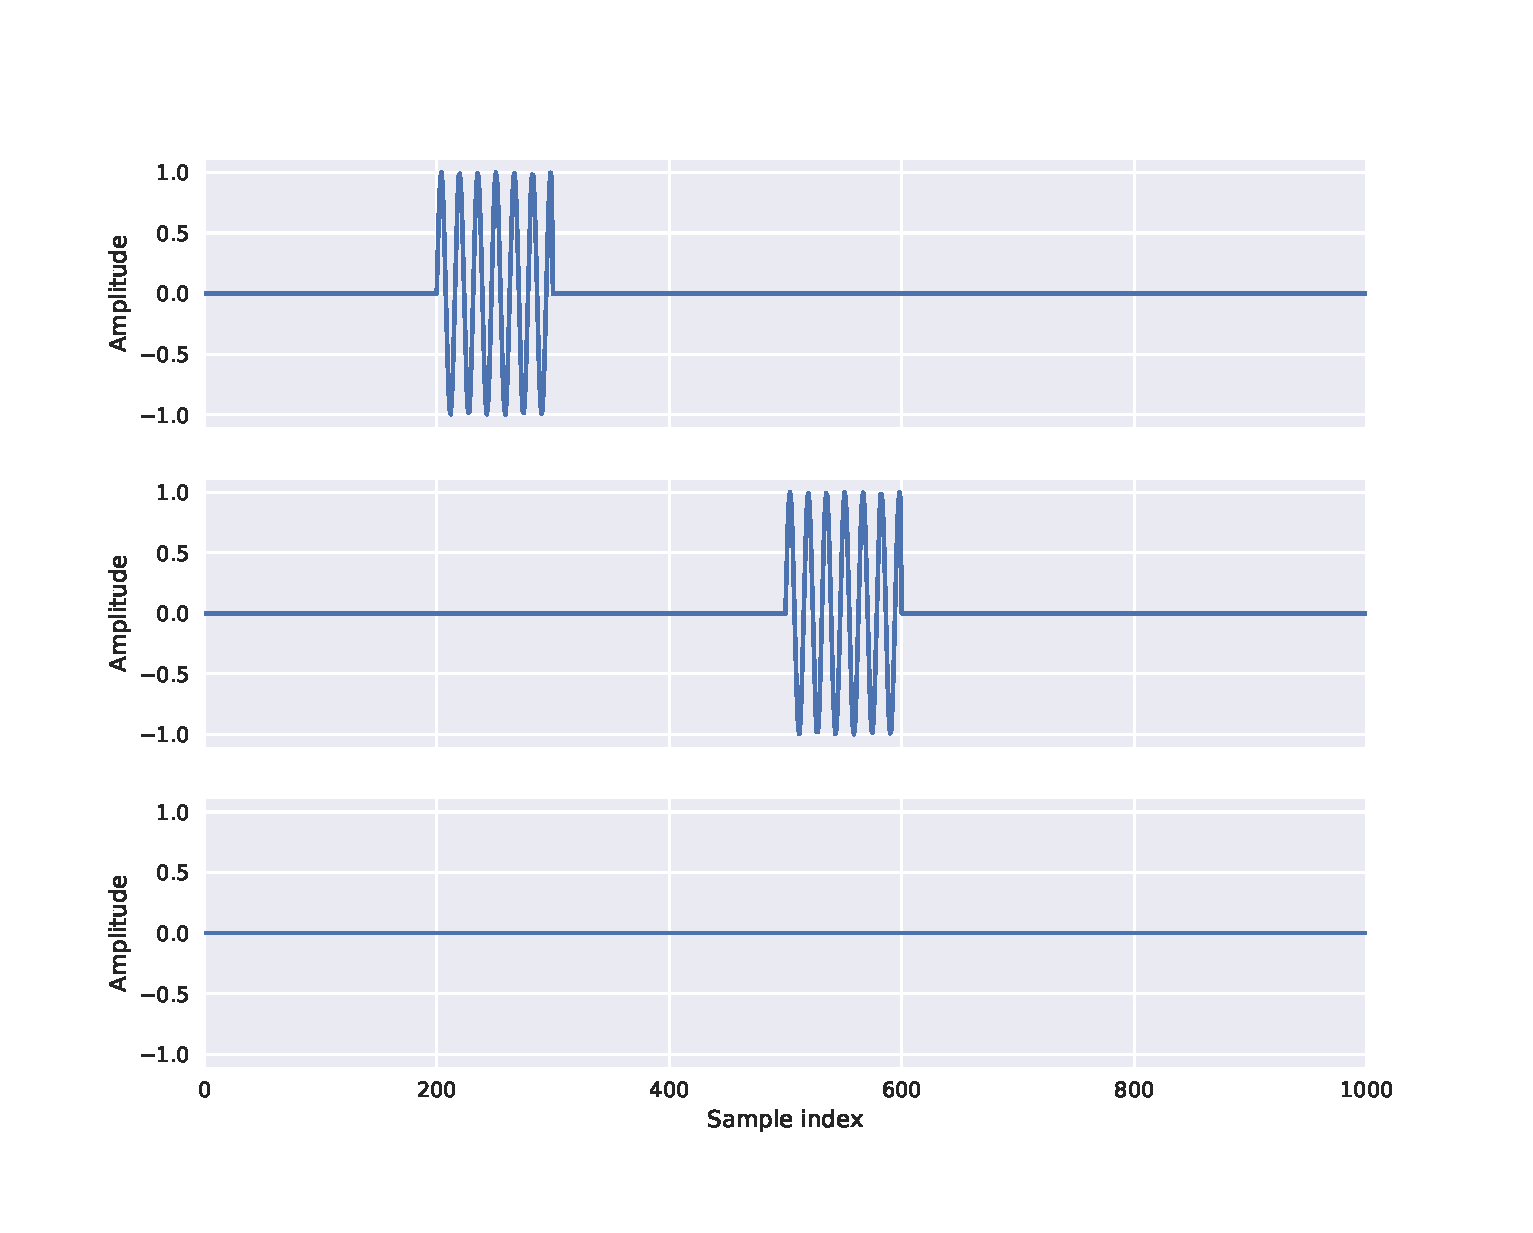
\includegraphics[scale=0.5]{figs_temp/mixing0}
	\caption{Analysis pulse $x_T(t-\tau)$ (top), received pulse $y(t)$ (mid) and multiplication output $x_T(t-\tau)y(t)$ (bot). As the signals do not overlap the multiplication yields only zero values.}
	\label{fig:mix0}
\end{figure}

\begin{figure}[h]
	\centering
	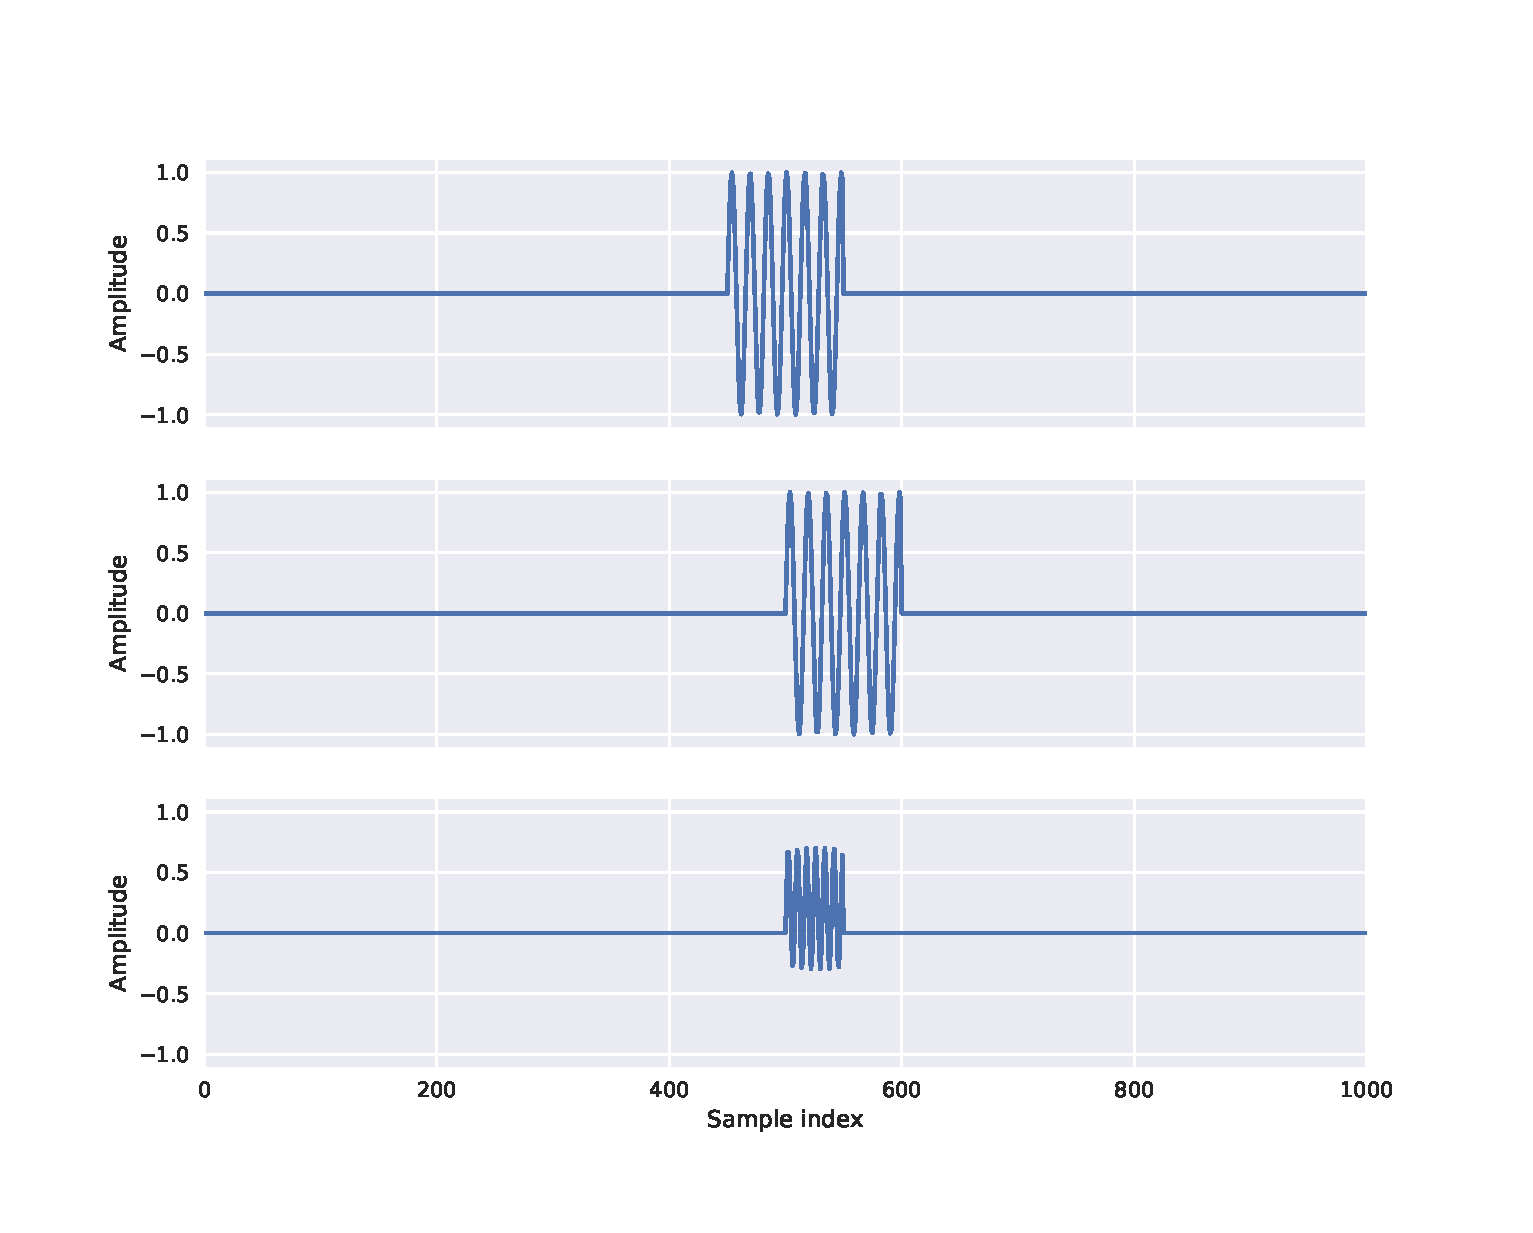
\includegraphics[scale=0.5]{figs_temp/mixing1}
	\caption{Analysis pulse $x_T(t-\tau)$ (top), received pulse $y(t)$ (mid) and multiplication output $x_T(t-\tau)y(t)$ (bot). The overlapping signals produce non-zero values after multiplication.}
	\label{fig:mix1}
\end{figure}

\begin{figure}[h]
	\centering
	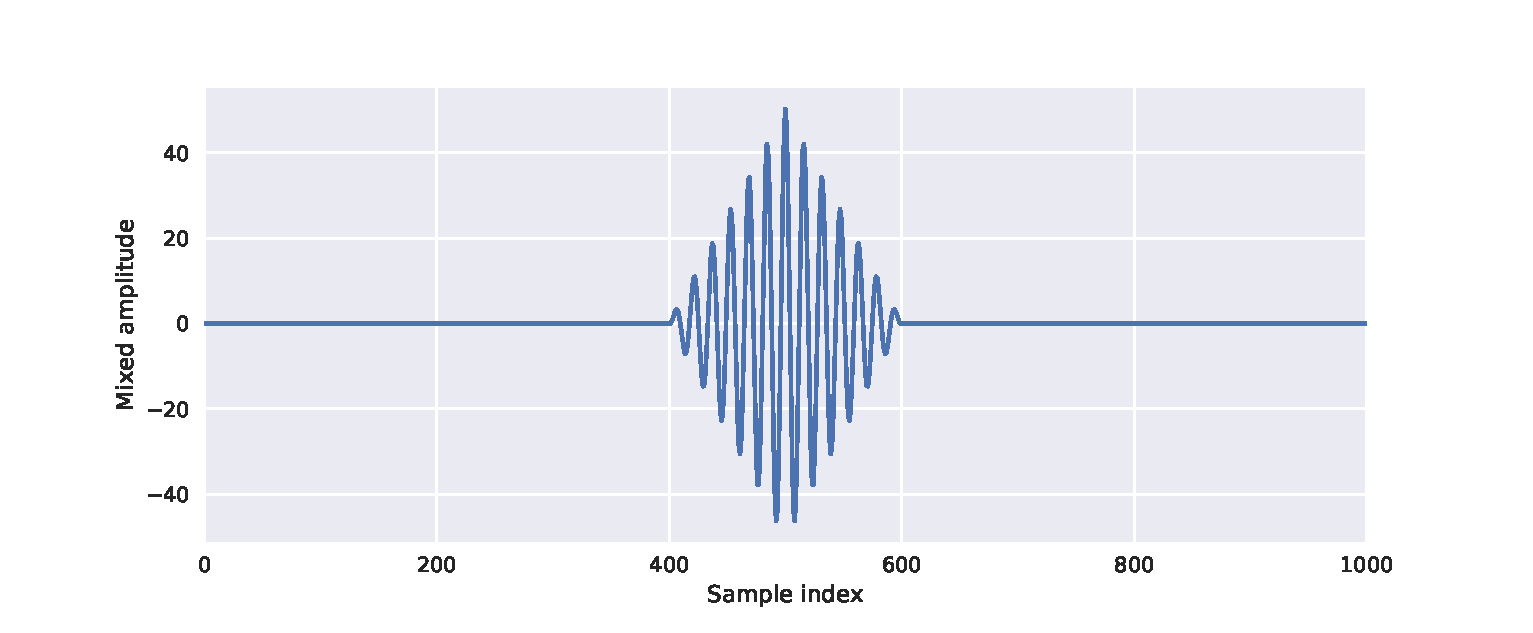
\includegraphics[scale=0.5]{figs_temp/mixing2}
	\caption{By integrating the multiplication at each delay the mixing output $m(\tau)$ is produced.}
	\label{fig:mix2}
\end{figure}

\begin{figure}[h]
	\centering
	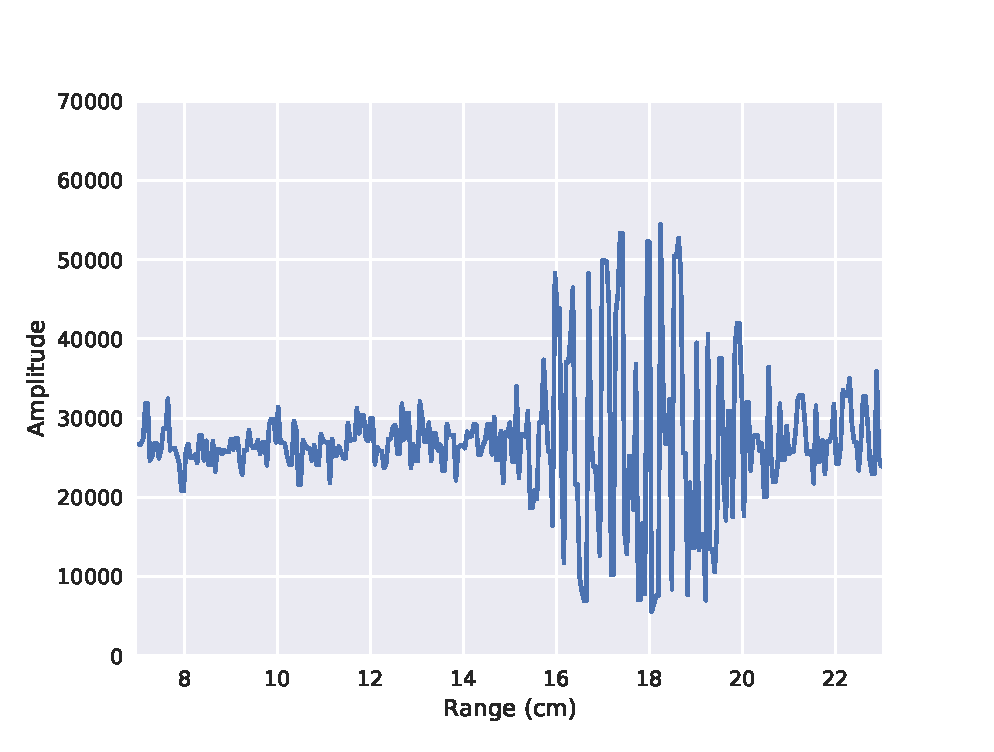
\includegraphics[scale=0.7]{figs_temp/single_sweep_raw}
	\caption{A single radar sweep which has been measured from 7 to 23 cm. The largest amplitude at around 18 cm. suggests there is some object present at that distance from the sensor.}
	\label{fig:single_sweep_raw}
\end{figure}

\section{IQ Demodulation}
\label{sec:iq}

Even though single-antenna receivers have no angular resolution, it was shown above that the returning signal carries useful information. By measuring the temporal shift from transmission to reception we can calculate the distance to a scatterer, and by examining the phase shift between pulses we may find the \gls{bf} and thus the radial velocity of the scatterer. Finally, the scatterers dielectric properties are brought forward through the \gls{rcs}, showing up as a scaling factor after analog convolution. 

Although the raw signal produced by analog convolution shown in \ref{fig:single_sweep_raw} holds the information we are interested in, it has commonly low \gls{snr} \citep{richards_2014} and holds the carrier frequency as can be seen in \ref{eq:n0}-\ref{eq:n2}. Instead, some transformation of the raw signal is usually performed. In this work we are particularly interested in resolving small Doppler shifts, and thus we wish to closely monitor phase shifts from one measurement to the next. One effective method focusing on accurate phase tracking involves splitting the signal into its \emph{In-phase} and \emph{Quadrature} (\gls{iq}) components. 

The In-phase channel mixes the raw signal with an oscillator at the carrier frequency $f_c$, and the Quadrature channel with the same frequency but with a $90^\circ$ phase shift from the I channel. After low-pass filtering, the \gls{iq} components are intepreted as a complex number $I(t) + jQ(t)$. \gls{iq} demodulation shifts the information bearing part of the mixed signal to baseband, meaning that an echo waveform on form $A(t)\sin(2\pi f_c t + \phi(t))$ after demodulation has form $A(t)e^{j\phi(t)}$, effectively eliminating the carrier frequency. Thus, after analog convolution and \gls{iq} demodulation we obtain a set of complex range measurements that we will denote as a \emph{radar sweep}. 

The details of this demodulation scheme can be found in the appendix. In figure \ref{fig:single_sweep_iq} the amplitude of a radar sweep is shown for data captured using the same measurement setup as in figure \ref{fig:single_sweep_raw}. Although the amplitude may be useful, the real power of splitting the signal into its I and Q constituents come from its phase tracking capabilities, as the phase is vastly more sensitive to small changes in range than the amplitude \citep{lien_gillian_karagozler_amihood_schwesig_olson_raja_poupyrev_2016}.

% Is this good enough?
% TODO: Incorporate more of what is written below. Intermediary frequency? Discuss with Peter. 


%A common type of data when working with radar signal processing is in-phase and quadrature-phase data (IQ-data). IQ-data is represented as complex numbers, and a radar sweep consists of several such complex numbers - one for each investigated range. The process of obtaining IQ-data is often referred to as IQ- or quadrature demodulation, and is described in appendix .... The usefulness of this type of data lies in that it contains explicit information about the amplitude, $A(t)$, and phase, $\theta(t)$, in equation \eqref{eq:raw_sweep} \citep{richards_2014}. To obtain the amplitude for a sweep, $s$, one simply computes the absolute value for each complex number in $s$. The amplitude plot is a good way to visualize at what ranges objects are present. Figure \ref{fig:single_sweep_iq} illustrates such a graph where the same measurement setup as in figure \ref{fig:single_sweep_raw} has been used. Similarly, a phase curve can be obtained by computing the phase in each point.

%In many applications, the phase information in IQ-data is used when small changes in the radar signal need to be detected, (Mention a case such as recording over grass...) as the phase is more sensitive to changes than the amplitude \citep{lien_gillian_karagozler_amihood_schwesig_olson_raja_poupyrev_2016}. If an object is detected at distance $r(t_1)$ from the radar at time $t_1$, and shortly thereafter, the object is moved to distance $r(t_2)$, the corresponding difference in phase will be
%\begin{equation}
%	\label{eq:phase_diff}
%	\Delta\phi(t_1, t_2)=\frac{4\pi}{\lambda}(r(t_2)-r(t_1)) \quad\quad \textrm{mod 2$\pi$}
%\end{equation}
%By having a sampling frequency which is too low, the range difference in $\eqref{eq:phase_diff}$ could potentially become very big, and the phase difference would fluctuate over time and be incomprehensible.

%In the case of material classification, a high sampling frequency is highly beneficial. When moving across surfaces characterized by tiny details, a high sampling frequency is essential in capturing the shapes of these.

\begin{figure}[h]
	\centering
	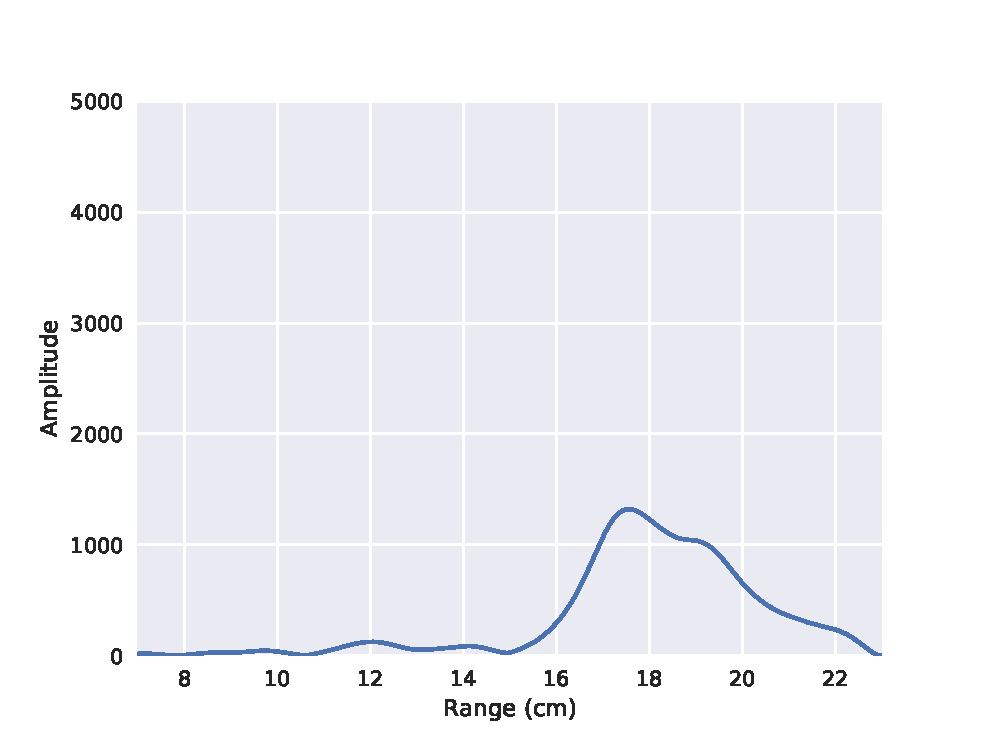
\includegraphics[scale=0.7]{figs_temp/single_sweep_iq}
	\caption{Visualization of an amplitude function derived from IQ-data.}
	\label{fig:single_sweep_iq}
\end{figure}

%For a thorough description of how IQ-data is derived, see appendix ...











%
%



% Data acquisition and preprocessing
\chapter{Data acquisition and preprocessing}

Having reliable data is a fundamental requirement in building a good model. In this chapter we describe the data measurement setup and the data acquisition process used in capturing the dataset used for surface classification. 

\section{Data representation}

A common representation of data acquired by multi-antenna radars is the \emph{datacube} \citep{richards_2014}. The first dimension of the datacube consist of the range measurements. Range measurements are formed from estimating the time-of-flight of a returning wavelet from a target scene. This process forms the shortest time frame possible with sample spacing on the picosecond scale for millimeter-wave radar, and is thus commonly referred to as the \emph{fast time} scale. With sampling frequency $F_s$ new measurements are produced every $1/F_s$ seconds. This sequence of measurements form the second dimension. Due to its much slower rate (on the $1/F_s$ scale) it is referred to as the \emph{slow time} scale. Finally, the last dimension is constructed from the receiver indicies. This intuitively pleasing representation of data acquired by radar arrays are commonly referenced in journal papers when describing for instance beam forming or doppler processing algorithms \citep{gentile_donovan_2018}. 

In this report systems with only a single receiving antenna is used generating data with only fast and slow time dimensions. However, in this project two such systems are uused in parallell, but not synchronized to one another. This means that the sensors take turn measuring their surroundings as opposed to listening to the same returning wavelets. Thus, it would be incorrect to treat these two sensors as the third dimension of datacubes, which would indicate that the two sensors are synchronized.

Instead, we may just as well concatenate the two sensor outputs to form a \emph{data matrix}. If the contents of one radar sensor output with fast time index $d=1...Z$ and slow time index $t=1...Q$ is described with $r(d,t)$, we form a data matrix $\mathbf{R}$ with sensors $r_1(d,t)$ and $r_2(d,t)$ through

\begin{equation}
	\mathbf{R}= 
	\begin{bmatrix}
		r_1(0,0) & r_1(1,0) & \cdots & r_1(Z,0) & r_2(0,0) & \cdots & r_2(Z,0) \\
		r_1(0,1) & r_1(1,1) & \cdots & r_1(Z,1) & r_2(0,1) & \cdots & r_2(Z,1) \\
		\vdots &  \vdots & \ddots & \vdots & \vdots & \ddots &  \vdots \\
		r_1(0,Q) & r_1(0,Q) & \cdots  & r_1(Z,Q) & r_2(0,Q) & \cdots  & r_2(Z,Q) \\
	\end{bmatrix}
	,
\end{equation}
or, more succinctly, as samples $r(n,t) = \mathbf{R}_{t,n}$ with $n=1...2Z$. Each collected data matrix is built up of 50,000 slow time samples, so that $Q=50000$.

\begin{figure}
	\centering
	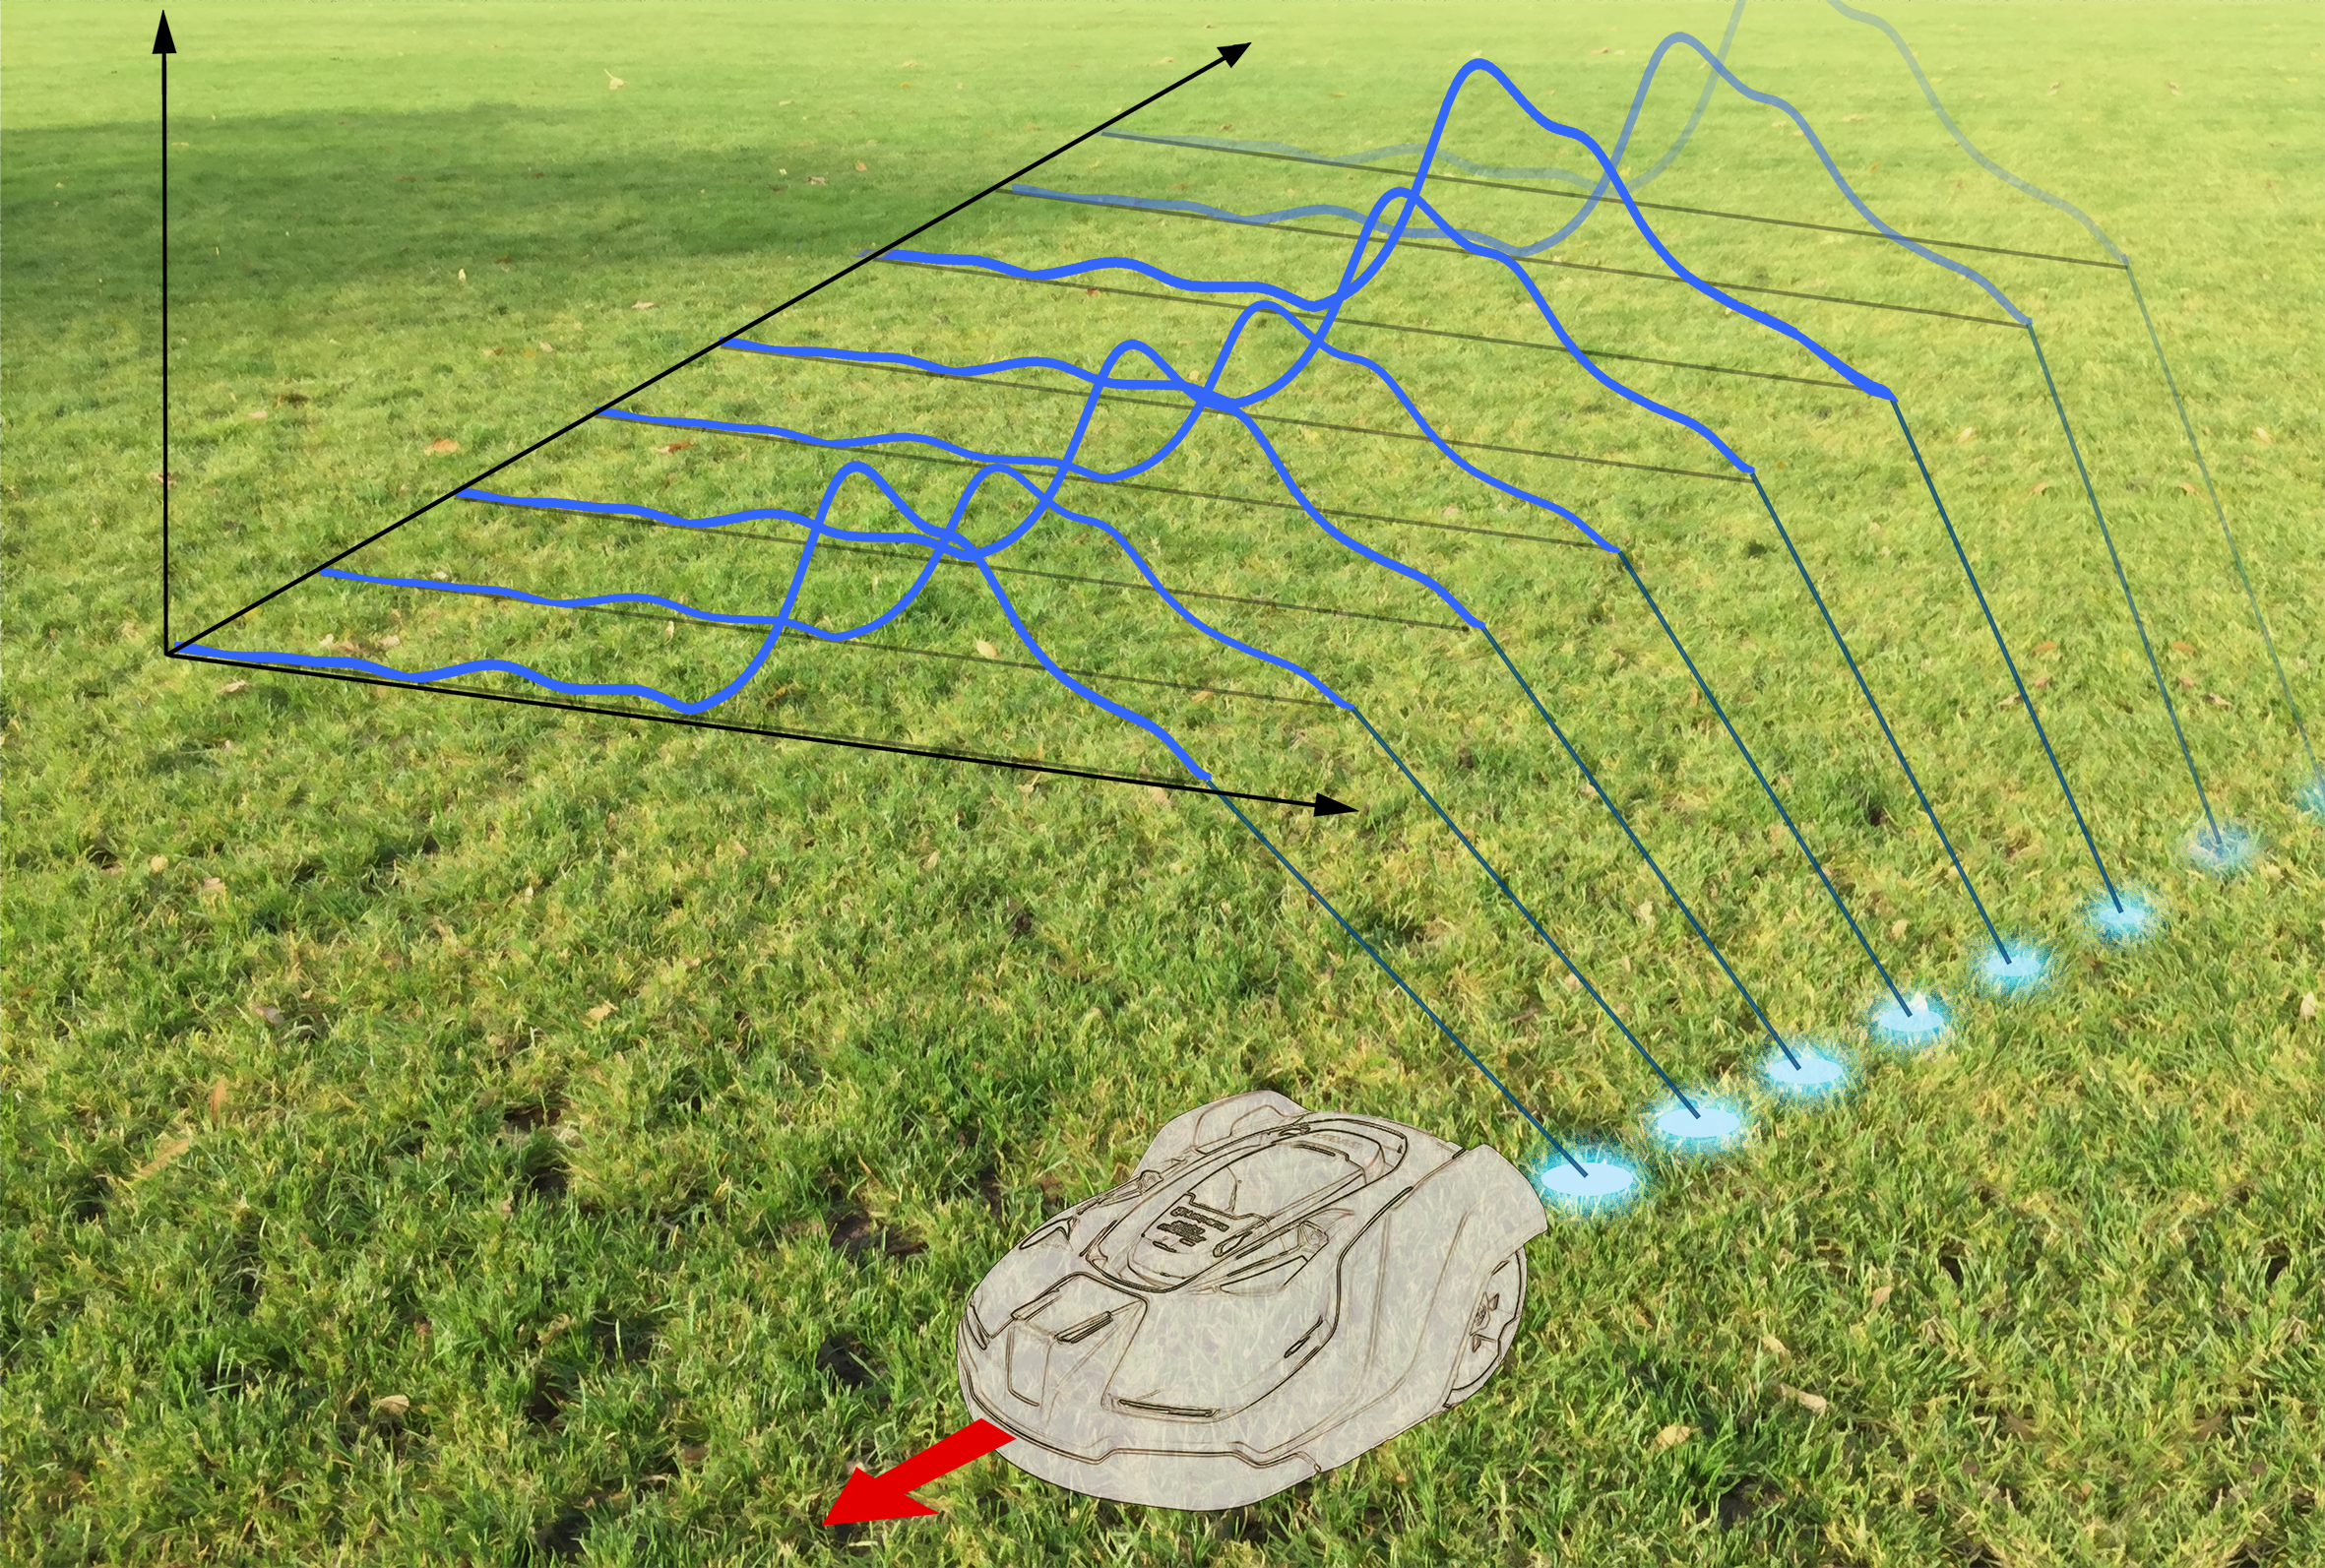
\includegraphics[scale=0.60]{figs_temp/data_collecting.jpg}
	\caption{Two sensors mounted at the front of a robot collect data while the robot is moving forward. Note that the collected data is split in its \gls{iq} components, whereas the image depicts its absolute values for the sake of clarity.}
	\label{fig:data_collecting}
\end{figure}

\section{Measurement Setup}

As mentioned above, two sensors each capture one data matrix per measurement session. Sensor data is acquired while the robot is moving at a constant pace, illustrated in figure \ref{fig:data_collecting}. Furthermore, two mounting angles are used, where one sensor is facing directly towards the ground while the other has a $22.5^\circ$ tilt forward. The reasoning behind this setup is for each sensor to capture different aspects of the surface below; the sensor placed flat downwards captures a larger component of the specular (mirror-like) scattering process from the ground plane, while the tilted captures more of the non-specular scatterers. 

This idea is illustrated in figure \ref{fig:reflections}. If we are presented with two surfaces of the same material but with different ruggedness, the two will still scatter differently in spite of their equivalent dielectric properties. The scattering processes considered in this work should be highly dependant on the surface structure, where the predictability (or the randomness) should vary from material to material. It is worth noting that the angular spread of the sensor is roughly $30^\circ$ \citep{acconeer_datasheet_a111}, meaning that a $60^\circ$ angle from the sensor is illuminated at once. 


\begin{figure}[h]
	\centering
	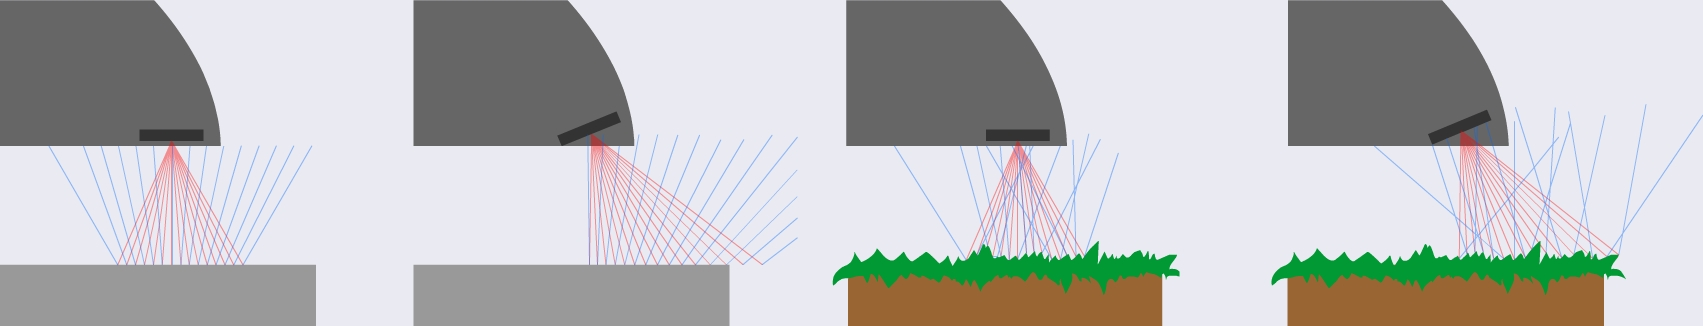
\includegraphics[scale=0.9]{figs_temp/reflections.jpg}
	\caption{Using two sensors mounted with different tilts, we can get information about a surface's roughness. For a smooth surface, the flat and tilted sensors yield a very different response, whereas for a rugged surface the responses are more similar.}
	\label{fig:reflections}
\end{figure}

A final consideration is that as the sensors are placed on the inside of the robot plastic chassis, there is a risk for interference between in the region between the plastic and the antenna. To avoid this a small mount was 3D-printed so that the distance to the plastic was $\lambda/4$. Doing this means that any waves propagating back and forth in this region interfere destructively due to the change in polarity and the superposition principle of electromagnetic radiation \citep{griffiths_2018}.

\section{Target Surfaces}
%TODO: Maybe cool figure with the surfaces. 

In this work we wish to see if we can create a binary classifier capable of distinguishing grass from non-grass surfaces. For the application of keeping a robot lawn mower in bounds, it is natural to select other surfaces that commonly borders lawns. With this in mind the surface selection is presented in table \ref{tab:count}, as well as the number of measurement sessions per surface. Each sessions were taken either on different days, or different locations. Note that the total sampling time amounts to $50,000\times42/(F_s\times60)=175$ minutes.

\begin{table}
\begin{center}
	\begin{tabular}{|c|c|}
		\hline
		\rowcolor{gray!150}\color{white}\textbf{Surface} & \color{white}\textbf{Num. sessions} \\
		 Grass & 18 \\
		 \rowcolor{gray!25} Asphalt & 6 \\
		 Gravel & 6 \\
		 \rowcolor{gray!25} Soil & 8 \\
		 Tiles & 4 \\ \hline
		 \rowcolor{gray!25} Total & 42 \\
		 \hline
	\end{tabular}
\end{center}
\caption{Measured surface types and number of measurement sessions per surface type.}
\label{tab:count}
\end{table}

\iffalse
\begin{table}
\begin{center}
	\begin{tabular}{|c|c|}
	  	\hline
	  	\cellcolor{gray!150}\color{white}\textbf{Setting} & \cellcolor{gray!150}\color{white}\textbf{Value} \\
	 	 Wavelet duration & 50 ps \\
	  	\cellcolor{gray!25}Sampling frequency & \cellcolor{gray!25}200 Hz \\
	  	Range interval & 7 to 23 cm \\ 
		\hline
  	\end{tabular}	
\end{center}
\caption{Sensor settings.}
\label{tab:sensor_settings}
\end{table}
\fi

\section{Measurement Settings}

The Acconeer \gls{pcr} system has a number of user-defined settings. In this section a few key parameters of these are discussed, namely the range interval sampled, the slow time sampling rate and the wavelet duration. Although finding the appropriate sensor settings requires some level of trial-and-error due to hardware and software limitations, a good starting point can be found using a theoretical perspective. 

\subsection{Sampling rate}
When working with radars and moving targets it is important to select a frequency capable of resolving the maximum speed that the target can have. If a too low frequency is used, aliasing occurs distorting the frequency spectrum \citep{lindgren_rootzeŽn_sandsten_2013}. In order to assure that aliasing does not occur, one must select a sampling rate $f_s$ at least twice the received maximal frequency component $f_{max}$. This limit, commonly known as the Nyquist limit \citep{proakis_manolakis_1995}. From section \ref{sec:doppler} we found that the velocity $v$, the carrier wavelength $\lambda_t$ and the \gls{bf} $f_d$ are related through $v \approx \lambda_tf_d/2$. Combining these two, we require from the sampling rate $F_s$ that 

\begin{equation}
\label{eq:nyquist}
		F_{s} \geq 2f_{max} 
		= 2f_d 
		\approx \frac{4v}{\lambda_t}.
\end{equation}

The velocity above is the \emph{radial} velocity. In the measurement setup depicted in figure \ref{fig:sensor_placement}, a vehicle is moving forward with constant speed $v_0$ having a sensor mounted at the front with a 22.5 degree tilt and a 60 degree angular spread. The maximal velocity component that is orthogonal to the sensor occurs at the far end of the radar's view at $22.5^\circ + 30^\circ = 52.5^\circ$ tilt. With $\lambda_t=c/f_t=0.005$ m and the maximum orthogonal velocity component $v_{\perp, max}$ the requirement above becomes

\begin{equation}
	F_s \geq 
	\frac{4v_{\perp, max}}{\lambda_t}
	= \frac{4v_0\sin(52.5^\circ)}{\lambda_t} 
	\approx 190 \text{ Hz}.
\end{equation}

Thus, in order to avoid aliasing, the sampling rate $F_s$ should be at least 190 Hz. 


\begin{figure}[h]
	\centering
	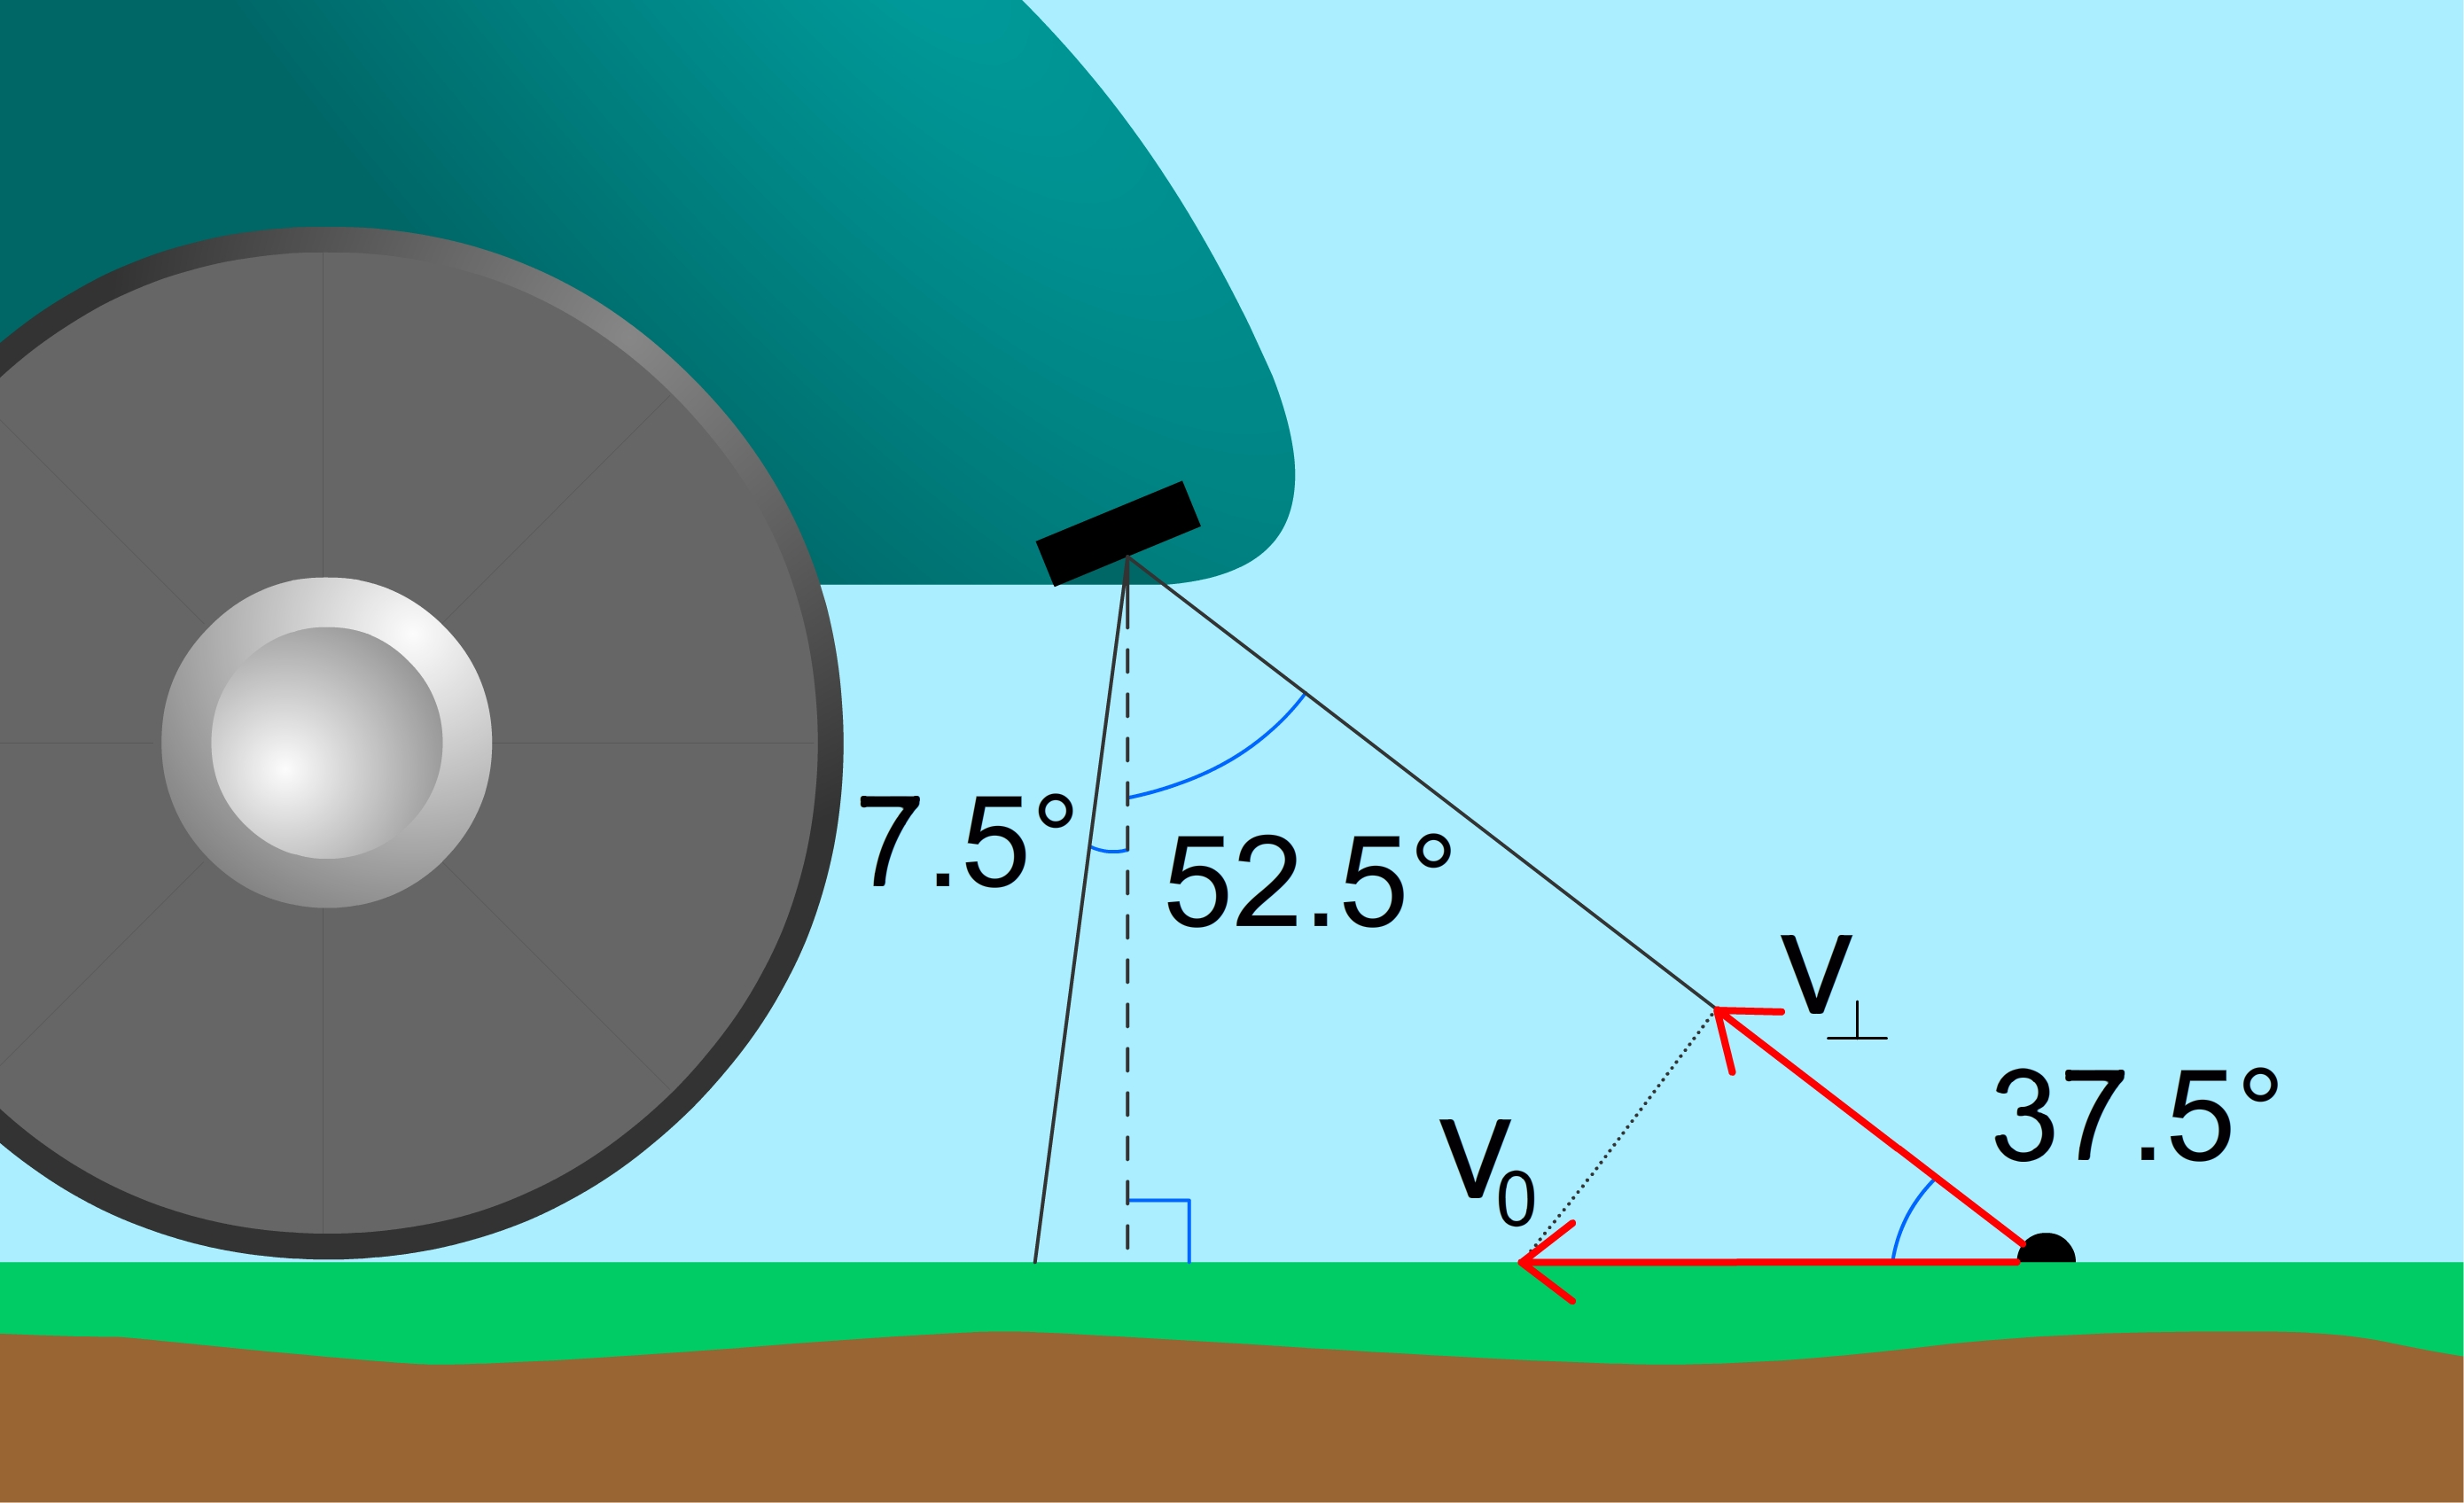
\includegraphics[scale=0.30]{figs_temp/sensor_placement.jpg}
	\caption{Sensor placement in robot chassis. The figure indicates the furthest point visible by the radar.}
	\label{fig:sensor_placement}
\end{figure}
\subsection{Wavelet Duration}

%TODO: Introduce some brief bandwidth concepts here 
The length, or duration, of the transmitted wavelet pulses in a \gls{pcr} system determines the bandwidth. 

The frequency is essentially set for the system used at around 60 GHz without any significant leeway. The duration may however be chosen somewhat freely. Selecting a longer wavelet means transmitting more energy and thus receiving a signal with better SNR. A shorter wavelet has worse SNR, but is capable of resolving finer details of the target. Thus, the wavelet duration parameter becomes a tradeoff between resolution and SNR. One may start with a short wavelet and increase its duration until a reasonable SNR is obtained.  

\subsection{Range Swath}

Finally, the radar measures power over some range interval, also called the \emph{range swath} \citep{richards_2014}. Again, a tradeoff appears. If a short interval is selected we can increase the sampling rate and still stay within the allowed hardware transmission speed limits. However, if the interval becomes too short we may miss useful information we could have collected outside the chosen interval. Thus, a reasonable strategy is to select the most critical range interval and then increase the sampling frequency to its hardware allowed limit. As the distance to the surface plane was roughly 12 cm the furthest distance illuminated is $12/\sin(37.5^\circ)\approx 20$ cm. We should therefore at least have a range swath spanning this region. 

The values chosen for the three parameters are summarized in table \ref{tab:sensor_settings}.

\begin{table}
\begin{center}
	\begin{tabular}{|c|c|}
	  	\hline
	  	\cellcolor{gray!150}\color{white}\textbf{Setting} & \cellcolor{gray!150}\color{white}\textbf{Value} \\
	 	 Wavelet duration & 50 ps \\
	  	\cellcolor{gray!25}Sampling frequency & \cellcolor{gray!25}200 Hz \\
	  	Range interval & 7 to 23 cm \\ 
		\hline
  	\end{tabular}	
\end{center}
\caption{Sensor settings.}
\label{tab:sensor_settings}
\end{table}

\section{Downsampling}
\label{downsampling}

In information theory we interpret and quantify random variables by how unpredictable or unstructured observations of the random variables are \citep{anderson_johnnesson_2006}. Using such a framework, we could argue that variables that contain the same information as others in the same set are obsolete and can be discarded \citep{hyvasrinen_karhunen_oja_2004}, as we ideally we want data that contain information not found elsewhere in the set. 

Using the settings in table \ref{tab:sensor_settings} we obtain 331 range samples per radar measurement in the 7-23 cm range, which means samples are spaced by $(230-70)/331\approx0.48$ mm. Observing a typical radar sweep in figure \ref{fig:single_sweep_iq} we note that points are very closely related on a small range scale, and nearly identical if we were to examine them on a sample by sample basis. Hence individual samples are low on information, and we can downsample by some integer factor $D$, and an offset $F$ without significant loss of information.

Downsampling measurements $r_1(d,t)$ and $r_2(d,t)$ by a factor $D$ with offset $F$ can be expressed as

\begin{equation}
	r_{1,D, F}(d, t) = r_{1}(F+dD,t), 
	\quad \text{and} \quad r_{2,D,F}(d,t) = r_{2}(F+dD,t)
\end{equation}
and the data matrix $r_{D,F}(n,t)$ is formed correspondingly.

\section{Sweep Normalization}

Radar gain can vary significantly from one sensor to the next. This means that faced the same surface, two sensors may exhibit a similar sweep structure but scaled differently. Assuming a models training data has been collected with one sensor, it could therefore be difficult to successfully perform classifications with the same model using a sensor which has a different gain. This is due to the fact that a linear scaling difference between two sensors behaves nonlinearly in the prediction output, due to nonlinearities both in the feature extraction process as well as in the classification process.

A way to overcome this issue is to perform sweep normalization as a preprocessing step. There are multiple ways of performing such a normalization. A simple strategy is to simply divide each sweep with its maximum absolute value. While this may intuitively seem like a good idea, it eliminates signal evolution structures between consecutive captured sweeps - if three consecutive sweeps vary in received signal strength we wish to capture such a behaviour. 

A better solution is to instead have the normalization method depend on several consecutive sweeps. Normalizing using multiple sweeps thus maintain some of their relative amplitude structure. Constructing a set of smaller data matrices with index $m$, consisting of $r_D(n,mT + t)$ for $t=0\text{ }...\text{ }T-1$ for $T$ consecutive sweeps, we can average over the average amplitude in the $m$'th data matrix to form scaled, downsampled data $x(n,m,t)$ through

\begin{equation}
	x(n,m,t) = 
	\frac{r_{D}(n,mT + t)TK}
	{\sum_{n=0}^{K-1}\sum_{\tau=0}^{T-1}|r_{D}(n,mT + \tau)|}.
\end{equation}

While this particular method to form data matrices $x(n,m,\tau)$ may seem odd at this point, we will see in the following chapter that it makes a lot of sense with the feature extraction framework used.


% Feature selection

\chapter{Feature Extraction}

In this chapter we describe our feature extraction process. This process is an intermediary step between data preprocessing and surface classification where we calculate metrics that are used for classification. After introducing some potential features we compare the accuracy of a few feature ensembles using a linear classifier to determine which ensemble should be used for further analysis.  

\section{Why Feature Extract?}

Machine learning algorithms fundamentally aim to extract useful patterns in data. In our case, data consist of the complex output of two radar receivers and the useful patterns we search for are patterns capable of distinguishing the surface type as either grass or non-grass. %One way to accomplish this would be to simply hand the raw \gls{iq} radar sweeps to a classifier and allow it to figure out structures in the data on its own. However, for small autonomous devices hardware capabilities are often limited and radar systems comparatively fast, making complete real-time classification of the entire bulk of acquired data cumbersome. 

We found in chapter 2 that a single radar sweep only provides information about ranges and reflectivities but cannot determine target velocities. Due in part to the normalization process done in the preprocessing step such measures alone will hardly suffice to make an efficient predictor. Instead information from several sequential sweeps should be used to generate a prediction. In order to make use of the information content present in the sequence of radar sweeps we have two main options. 

The first involves using a complex nonlinear machine learning algorithm, such as a deep neural network (\gls{dnn}) with a large number of hidden layers that figures out how to calculate efficient temporal metrics on its own, provided large bulks of unmodified data. Algorithms exist that indeed can learn to analyze frequency components, for instance for speech recognition \citep{graves_mohamed_hinton_2013}, but tend to be too computationally expensive to realistically implement when hardware is limited.

Instead we utilize that we know that taking the \gls{dft} in slow time provides velocity estimates for a given distance through \gls{bf}s, as was explained in \ref{sec:doppler}. The scaling of each frequency bin thus provides an estimate of the amount of velocity component at a given range. Such estimates are rich in information regarding the topography of a surface structure, as it accounts for the \gls{rcs} of a surface at different velocities and thus different angles of incidence. 

A second option is thus to utilize this knowledge and perform \emph{feature extraction}. By extracting a smaller set of features pertaining to the frequency content of the given data, we can significantly reduce the complexity of the model. Furthermore, the feature extraction process allows us to pinpoint what data characteristics we wish to monitor, and subsequently which data characteristics we believe are of value. This ensures that the machine learning algorithm generates its predictions using patterns in metrics selected by the authors, rather than finding patterns from raw input data. For these reasons the focus of this report is using feature extraction based machine learning. 

\section{Features}

Calculating velocity-based features require the use of a sequence of multiple sweeps. How long should one such sequence be? If $T$ radar sweeps are used per classification, the rate of classifications per second, $F_c$, produced relates to the sampling rate through
\begin{equation}
	\label{eq:classification_rate}
	F_c = \frac{F_s}{T}.
\end{equation} 

Hence, the parameter $T$ becomes a tradeoff between feature accuracy and classification rate. The more samples used per classification, the better the extracted features become at the cost of a lower classification frequency. Conversely, we may be able to generate feature estimates more rapidly by setting $T$ to a lower value, but will in the process end up with worse feature estimates. 

% Described in the preceding chapter...
%The reflectivity of a material, described by its dielectric constant, shows up in the obtained IQ-demodulated sweeps in the amplitude of the returning signals. Therefore it might seem like a good idea to simply measure the energy content of a sweep and use it as a feature. However, due to inconsistencies inbetween individual sensors, sweep normalization is performed as a pre-processing step rendering such calculations unusable. We are thus left with investigating the topography of the scene. 

In this section four different feature types are discussed aimed at capturing the geometric characteristics of a target surface. From a given data matrix $x(n,t)$ consisting of $T=25$ consecutive sweeps normalized as described in section \ref{sec:norm}, we construct for each feature type a corresponding feature vector. We can then concatenate different feature vectors to form longer sets of features as we please.  

\subsection{Envelope Estimation}

First of all we may characterize a sweep by its envelope form; that is, the shape of the absolute values of the radar sweeps. We do this by simply calculating the absolute value averages in slow time to construct the estimated envelope shape $\hat{x}(n)$ through
\begin{equation}
	\hat{x}(n) = \frac{1}{T}\sum_{t=0}^{T-1}|x(n, t)|.
\end{equation}

In figure \ref{fig:sweep_average} we see what such an averaging process yield. Individual variances are suppressed forming a stable estimate of the sweep shape. With $K$ fast time samples, the estimate of the expected envelope feature vector becomes 
\begin{equation}
	\mathbf{f}_{x} = 
	\begin{bmatrix}
		\hat{x}(0) & \hat{x}(1) & ... & \hat{x}(K-1)
	\end{bmatrix}.
\end{equation}

\begin{figure}[h]
	\centering
	\includegraphics[scale=0.7]{figs_temp/features/sweep_average}
	\caption{By averaging the absolute values of several consecutive sweeps we obtain a measure of the average sweep shape. The dashed line shows the average of individual absolute values of radar sweeps, shown as solid semi-transparent lines.}
	\label{fig:sweep_average}
\end{figure}


\subsection{Fourier Transform}

As discussed in section \ref{doppler} we can relate the velocity of a scatterer to its \gls{bf} through \eqref{eq:dopp}. When an entire target scene is illuminated, computing a \gls{dft} in the slow time domain thus provides a \emph{velocity profile} of the scene at every range, indicating the amount of each velocity is present for the range in question. Due to the sampling settings outlined in chapter \ref{ch:3}, no significant aliasing in the frequency spectrum should occur in theory, as the sampling rate was set with the Nyquist criterion in mind. In figure \ref{fig:fft} the \gls{dft}s of radar \gls{iq} data are shown for all surface types considered in this work. For visualization purposes the square root of the absolute values of the \gls{dft} are shown. For grass (the top two plots), the frequency content is contained mainly in the vicinity of the zero-frequency bin, while the other materials have larger components at higher frequencies. %The \gls{rre} assumes that a scatterer is radiating isotropically. If radiation instead can be regarded to be specular in nature, the \gls{dft} provides a good measure of the surfaces topography. %[Continu. %[Continue and add a source]

%While traversing a static surface at a constant speed, one could think of it as the details on the surface, such as small rocks, are moving closer to the radar sensor. As discussed in section \ref{doppler}, this alters the frequency of the transmitted signal according to the Doppler effect, and the radar detects beat frequencies, corresponding to the frequency shifts. Depending on the surface's characteristics, the doppler frequencies may vary. 

%One way to obtain the the frequency contents is by means of the \gls{dft}. In figure \ref{fig:fft}, typical \gls{dft}s are shown for all materials. The figure is intended to show differences in the \gls{dft}s. Hence, to make the difference more clear, the squre root of the \gls{dft}s have been plotted. For grass (the top two plots), it can be seen that the frequency content is contained mainly at the zero frequency and close to it. The other materials contain slightly higher frequency content as well. Gravel, in particular, differs a lot from the other materials with a wide variety of frequency components.


% ¤¤¤¤¤¤¤¤¤¤¤¤¤¤¤¤¤¤¤¤ Comments ¤¤¤¤¤¤¤¤¤¤¤¤¤¤¤¤¤¤¤¤¤i
% is x the small or large data matrix? Here it is both...
% I think the notation looks strange here...
% Instead just write the DFT? 

%As for the feature vector, a data matrix consisting of $T$ sweeps is selected. Viewing this as a matrix with elements $x(n,t)$, we can compute a $k$-step Fourier transform for each range, $n$, and sample index $m$, as

As for the feature vector, a $T$-step DFT along the slow time axis is first computed for each range, $n$, as
\begin{equation}
	\mathbf{d}_n=\text{DFT}\big\{x(n,t)\big\}_t =  \sum_{t=0}^{T-1}x(n,t)\exp\Big(-2\pi i\frac{kt}{T}\Big), \quad k=0,...,T-1.
\end{equation}

After this, the transformations for all ranges are concatenated into a one-dimensional feature vector. This feature vector must be real-valued, as the machine learning classifiers considered in this work use real-valued inputs. The feature vector is formed by taking the absolute values of the frequency components through
\begin{equation}
	\textbf{f}_{f}=\begin{bmatrix} |\mathbf{d}_0|^* & |\mathbf{d}_1|^* & \hdots & |\mathbf{d}_K|^* \end{bmatrix},
\end{equation}
where $|\cdot|^*$ denotes elementwise absolute values, and $K$ is the number of fast time samples.    


% This section is weirdly written imo 
%An important remark to make is that under the assumption that the autocovariance function of a process $y_t$ decays sufficiently fast, it is closely related to the Fourier transform of the process. The Wiener-Khinchin theorem states that \citep{lu_vaswani_2009} with certain properties\footnote{The process has to be wide sense stationary. The meaning of this is defined in section \ref{ACr}.}, a process, $y_t$, the Fourier transform of its autocovariance function, denoted $\phi_y(\omega)$, relates to the Fourier transform of the actual process according to \citep{jakobsson_2015}
%\begin{equation}
%	\phi_y(\omega) = \lim\limits_{N\rightarrow\infty}E\Bigg\{\frac1N\Big|\sum^N_{t=1}y_te^{-j\omega t}\Big|^2\Bigg\}=\lim\limits_{N\rightarrow\infty}E\Big\{\frac1N|Y_N(\omega)|%^2\Big\}.
%\end{equation}
%An alternative to studying the Fourier transform could therefore be to examine the autocovariance of time series of IQ data.

\begin{figure}[h]
	\centering
	\includegraphics[scale=0.55]{figs_temp/features/fft}
	\caption{For each material a \gls{dft} is computed over 128 sweeps in slow time. For visualization purposes the square root of the absolute values of the complex-valued \gls{dft} is shown, highlighting differences in frequency content of the different surfaces.}
	\label{fig:fft}
\end{figure}


\subsection{Autocovariance in Range}
\label{ACr}

% This is actually wrong... and not well written atm
% Tie this into preceding section instead. Autocov allows for calculating the number of lags.
%An obvious surface characteristic to ponder is roughness; while a tiled surface is typically very flat, grass is characterized by a random, unpredictable structure. It is reasonable to assume that there is more correlation between two closely spaced points on the tiled surface than there is on grass. This motivates us to study the autocovariance in slow time.

A second method to investigate time-domain dependencies is through the autocovariance function. This method adds the benefit of allowing for a specification of the number of covariance lags, $q$, which subsequently determines the number of features. Figure \ref{fig:autocorr_range} displays absolute values of autocovariances estimated from 5000 sweeps for all surface types considered. As the most even surface, the tiled pavement shows the highest autocovariances, whereas grass - the arguably most uneven surface - indicates a low autocovariance. It should be noted that since only absolute values are shown, phase information has been lost in this plot.

\begin{figure}[h]
	\centering
	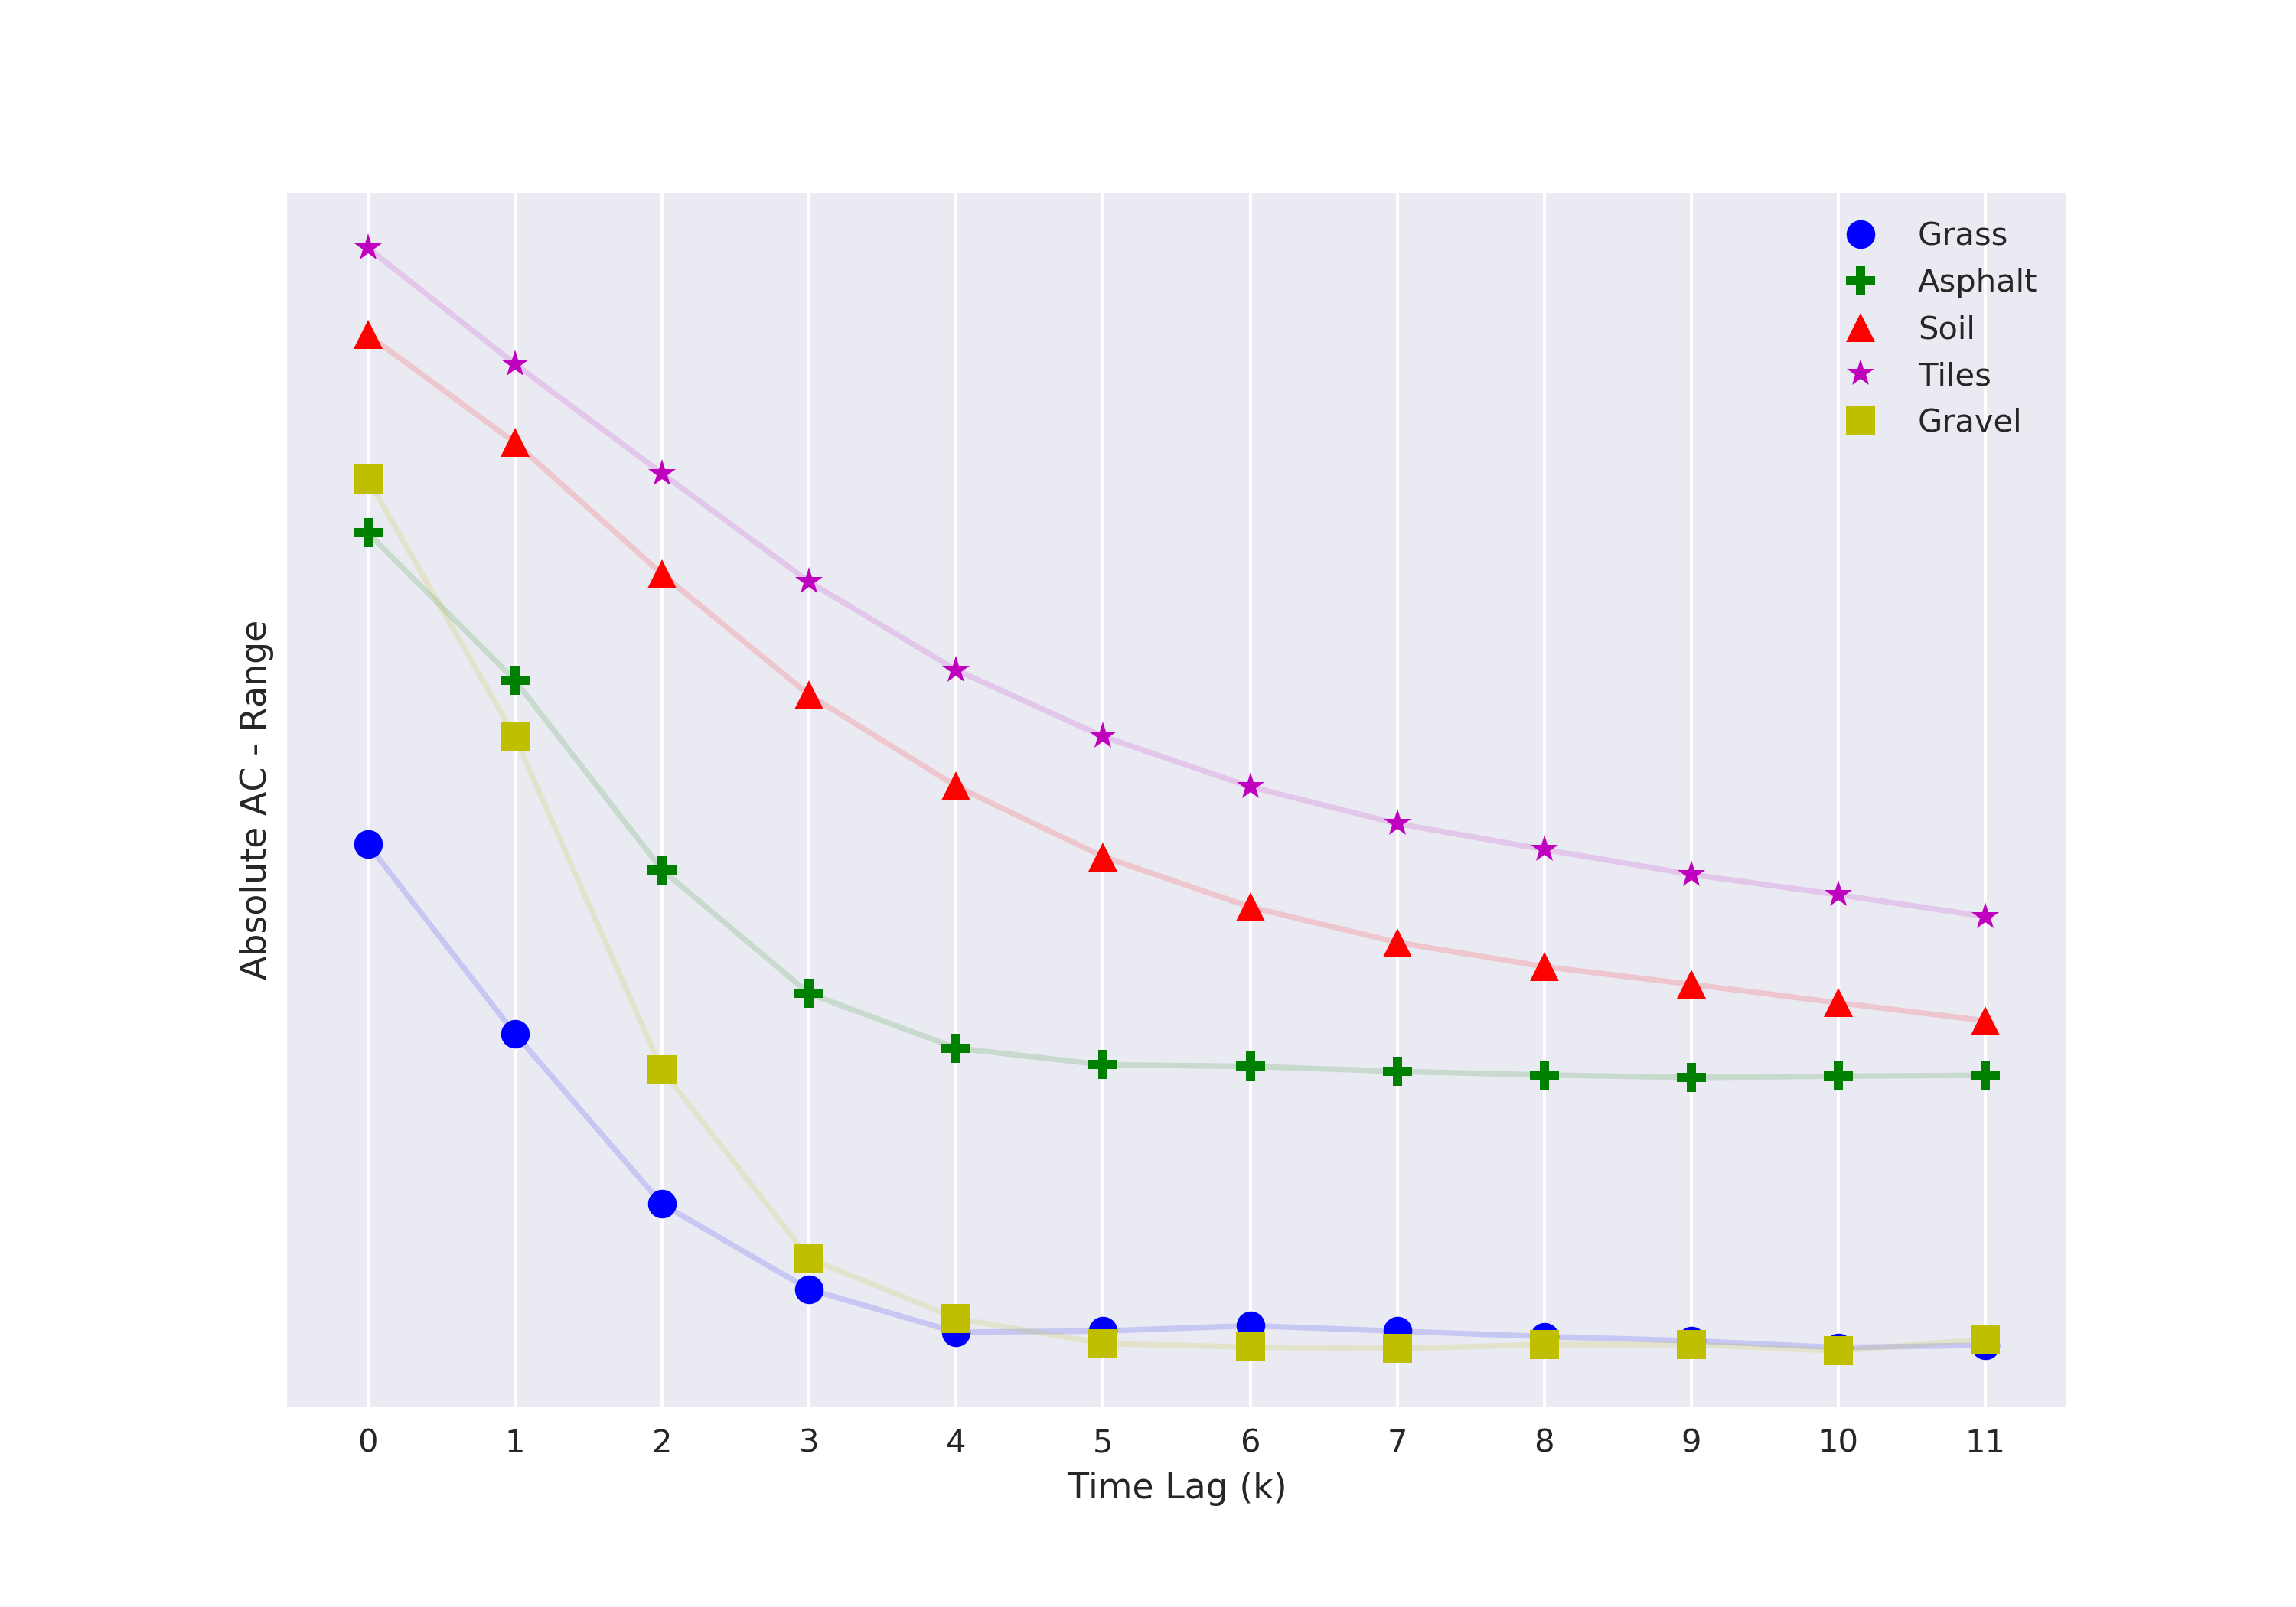
\includegraphics[scale=0.45]{figs_temp/features/autocorr_range.png}
	\caption{The first 11 autocovariance lags have been computed from a large number of slow time samples taken at roughly 14 cm for each surface considered in this work. The absolute values of the covariance lags are shown here for illustrative purposes. Note that only the zeroth lag is real-valued and that the others are complex valued.}
	\label{fig:autocorr_range}
\end{figure}

%We can regard the sequence $\{x(n,t)\}_{t=t_m}^{t_m+T-1}$ of measurements of range $n$ as samples from a stochastic process $X_{n,t}$ with the autocovariance function

%\begin{equation}
%	C_{XX}(n,t,s) = \text{Cov}(X_{n,t},X_{n,s}).
%\end{equation}


% We should maybe remove this tbh... or at the very least move it
%\noindent
%If we then can consider the process to have the following three properties:
%\emph{
%\begin{enumerate}
%	\item Constant finite mean
%	\item Autocovariance function only dependant on the difference $(s-t)$ and not on actual values of $s$ and $t$.
%	\item Finite variance
%\end{enumerate}
%}
%\noindent
%over the time interval $t_m$ to $t_m+T-1$, it can be regarded as a \emph{Wide-Sense Stationary} (WSS) process \citep{jakobsson_2015}. The first and second assumptions require the returning signal to carry some level of stability, which is reasonble considering the short time-frame $T/F_s$ considered. 


%We assume that $x(n,t)$ are samples from a stochastic process $X_{n,t}$ which is wide sense stationary (WSS) \citep{jakobsson_2015} over some short time $T/F_s$. Its autocovariance function for some range, $n$ may then be defined as
%\begin{equation}
%	r_n(k) = {\E}_t\big\{(X_{n,t} - \mu_n)^*(X_{n,t+k} - \mu_n)\big\}
%\end{equation}
%where $\mu_n=\E_t\{X_{n,t}\}$. We can form the (biased) estimate of the autocovariance function through

In order to have a reasonable classification rate, see \eqref{eq:classification_rate}, only $T=25$ sweeps are used for generating one feature vector. The biased estimate of the autocovariance function can be obtained through \citep{jakobsson_2015}
\begin{equation}
\label{eq:ac}
	\hat{r}_n(k) = \frac{1}{T}\sum_{t=k}^{T-1}\big(x(n,t) - \hat{\mu}_n\big)\big(x(n,t-k) - \hat{\mu}_n\big)^*
\end{equation}
where 
\begin{equation}
	\hat{\mu}_n = \frac1T \sum_{t=0}^{T-1}x(n,t).
\end{equation}

The bias in this estimate is completely inconsequential as all features later are normalized to zero mean unit variance. Autocovariance estimation through \eqref{eq:ac} is based on the assumption that $x(n,t)$ are measurements of a wide-sense stationary process. For a rough real-world terrain, this assumption is optimistic. However, the estimates may nonetheless make for useful metrics for classification as they feature slow time frequency content. The features may be formed as
\begin{equation}
	\hat{\mathbf{r}}_{k} = 
	\begin{bmatrix}
		\hat{r}_0(k) & \hat{r}_1(k) & ... & \hat{r}_{K-1}(k)
	\end{bmatrix}.
\end{equation}

Noting that the autocovariance sequence at 0 lag produces only real numbers, as any complex number $z = a + bi$ multiplied with its conjugate has zero imaginary part $\text{Im}(zz^*) = \text{Im}((a + bi)(a - bi)) = \text{Im}(a^2 + b^2) = 0$, we may form the full real-valued feature component for $q$ autocovariance lags $\mathbf{f}_{r}$ as
\begin{equation}
	\mathbf{f}_{r} = 
	\begin{bmatrix}
		\hat{\mathbf{r}}_{0}  & \text{Re}(\hat{\mathbf{r}}_{1} ) & \text{Im}(\hat{\mathbf{r}}_{1} ) & ... & \text{Re}(\hat{\mathbf{r}}_{q} ) & \text{Im}(\hat{\mathbf{r}}_{q} )
	\end{bmatrix}.
\end{equation}


%%%%% DISCUSSION OF AUTOCOV/CORR IMAGE %%%%%

%In figure \ref{fig:autocorr_range} the absolute values of calculated autocovariances are shown, estimated from 5000 slow time samples at a range of approximately 14 cm. Since only absolute values are shown phase information has been lost in this plot. We see that the grass surface has a dissimilar autocovariance sequence from the others, indicating that measuring autocovariance may be a good measure for distinguishing grass from other surface types.  

%From figure \ref{fig:autocorr_range}, we see that the the 1-step autocorrelation is what separates grass from other materials the most. For the feature vector we choose $q=2$, thus ncluding the variance as well as autocovariance steps 1 and 2 for the normalized sweeps.

%Figure \ref{fig:autocorr_range} illustrates the normalized autocorrelations for the different materials at a certain range. As expected, grass and tiles are two extremes in terms of roughness, and the other materials lie somewhere inbetween. Below, we explain how the autocovariance is formed in terms of features as preparation for the classifier.


\subsection{Autocovariance in Energy}

Although the sweep normalization process rendered absolute measurements of \gls{rcs} pointless, we are still able to investigate any time-dependent structure through the autocovariance function. First, we estimate the energy in each radar sweep $v(t)$ and the average energy $v_a(t)$ in $T$ number of sweeps, and then estimate the real-valued autocovariance sequence $h(k)$ as 
\begin{equation}
	v(t) = \frac{1}{N}\sum_{n=0}^{N-1}x(n,t)x^*(n,t)
\end{equation}
\begin{equation} 
	v_a = \frac{1}{T}\sum_{t=0}^{T-1}v(t)
\end{equation}
\begin{equation}
	h(k) = \frac{1}{T}\sum_{t=k}^{T-1}\big(v(t) - v_a\big)\big(v(t-k) - v_a\big)^*.
\end{equation}

As $h(k)$ only consist of real values, the energy autocovariance feature vector $\mathbf{f}_{h}$ is formed as
\begin{equation}
	\mathbf{f}_{h} = 
	\begin{bmatrix}
		h(0) & h(1) & ... & h(q-1)
	\end{bmatrix},
\end{equation}
where $q$ is the number of covariance lags. 

%We can also calculate the autocovariance function of estimated sweep energy. Although the sweeps are normalized in the preprocessing, we can investigate how the sweeps change over time. 

%The average energy in a sweep tells us how much energy is reflected back to the radar. Hence it can be regarded as a measure of how good of a reflector the underlying surface is. The energy depends on the shape of the surface, as well as its dielectric constant. Compared to other materials, grass has a very different surface shape, which potentially gives it a very different reflexivity. However, its dielectric constant could also vary a lot depending on whether it is wet or dry, making it hard to guess its reflective properties.

%By computing the average energy of single sweeps from different surfaces we see in figure \ref{fig:sweep_energy} that grass reflects much less energy. This indicates that the average sweep energy is a good feature for binary grass/not grass classification. However, in order to get a more robust measure of the average energy we do not only compute the average over selected range bins of a single sweep, but we average over a few consecutive sweeps as well. Mathematically, the feature we end up using becomes
%\begin{equation}
%	P(t_m) = \frac{1}{NT}\sum_{t=0}^{T-1}\sum_{n=0}^{K-1}x(n, t_m + t)x^*(n, t_m + t),
%\end{equation}
%where (describe variables)

%Despite the fact that the average energy appears to be a highly relevant feature, it is also much gain dependent, and conflicts with what is stated in section *reference to sweep norm.*. Therefore, if different sensors are to be used for training and future classifications, this feature will not be of any use.

\iffalse %%%%%%%
\begin{table}
\rowcolors{2}{gray!25}{white}
\begin{center}
  \begin{tabular}{|c|cccccc|}
\hline
    \rowcolor{gray!150}
		  & \color{white}\textbf{Abs.} & \color{white}\textbf{AC-E} & \color{white}\textbf{AC-R} & \color{white}\textbf{DFT} & \color{white}\textbf{Feats.} & \color{white}\textbf{SVM Acc. [\%]} \\
	  Config 1 & X &   &   &   & 28  & 92.23 \\
	  Config 2 & X & X & X & & 174 & 97.44 \\
	  Config 3 & & & & X & 700 & 97.37 \\
\hline
  \end{tabular}
\end{center}
	\caption{Three feature configurations of the four introduced features are compared. An X indicates that the feature is used in the configuration. Above, Abs indicate estimated envelopes, AC-E and AC-R autocovariances in energy and range, respectively, and DFT the discrete Fourier transform. Ideally we want as few features and as high linear separability, shown through an SVM accuracy score, as possible.} 
\label{tab:feat}
\end{table}
\fi
\begin{table}
\rowcolors{2}{gray!25}{white}
\begin{center}
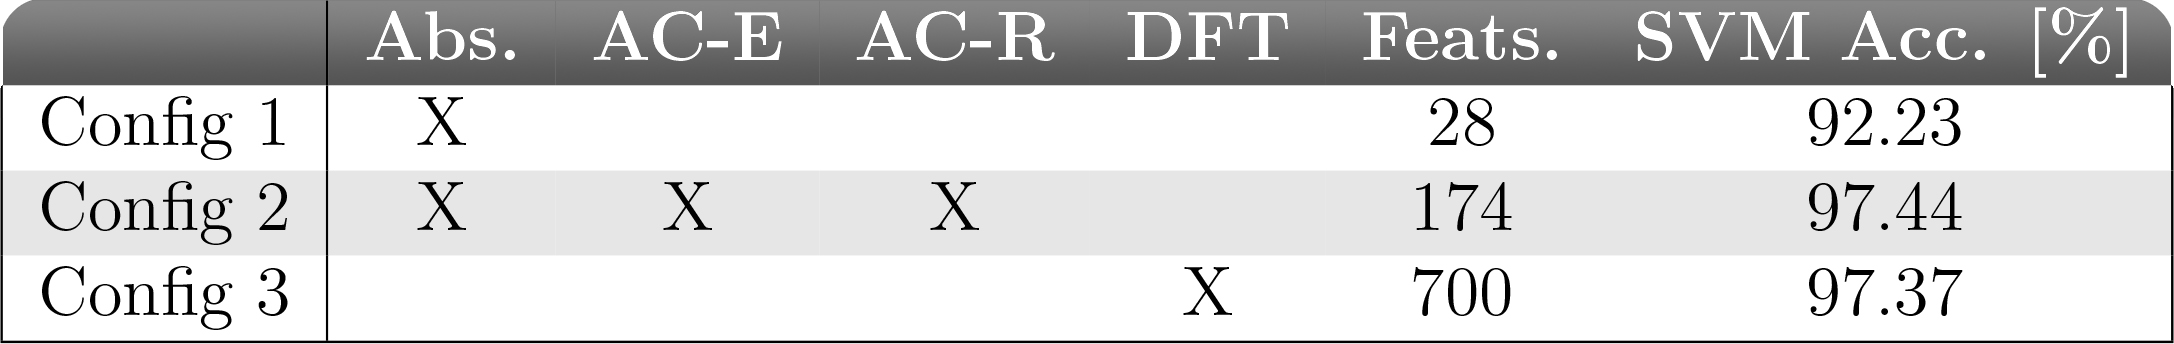
\includegraphics[scale=0.7]{figs_temp/table_config.jpg}
\end{center}
	\caption{Three feature configurations of the four introduced features are compared. An X indicates that the feature is used in the configuration. Above, Abs indicate estimated envelopes, AC-E and AC-R autocovariances in energy and range, respectively, and DFT the discrete Fourier transform. Ideally we want as few features and as high linear separability, shown through an SVM accuracy score, as possible.} 
\label{tab:feat}
\end{table}



% "The same model" is the hyperparameter optimized model we later get to, so the ordering is strange here. Numbers are off too.

\subsection{Reducing the Range Swath}

Before performing any feature processing, data is downsampled by a downsampling factor of $D=20$ as was described in section \ref{downsampling}. However, after examining a number of radar sweeps, it is clear that ranges below approximately 11 cm only contain little useful information. This can clearly be seen in the dark regions of the \gls{dft}s in figure \ref{fig:fft}. Similarly, little information is found at longer ranges. Therefore, we extract samples from an intermediate region when downsampling, modifying equation \eqref{eq:downsamp} to
\begin{equation}
	r_{1,D}(d, t) = r_{1}(50+dD,t), 
	\quad \text{and} \quad r_{2,D}(d,t) = r_{2}(50+dD,t)
\end{equation}
for $d=0,...,13$. With this definition, the downsampled radar sweeps consist of 14 evenly spaced range indices from ranges 9.4 to 21.9 cm. Thus, the resulting data matrix used for generating one set of features has $14\cdot 2$ complex ranges for the two sensors, and $T=25$ slow time sweeps. 

\section{Tested Feature Combinations}

Four different feature extraction methods have now been described - the average signal shape, the autocovariance in range and energy and the Fourier transform. Each method generates multiple features. However, we are not limited to feed our model with features taken from a single one of the methods. In table \ref{tab:feat}, results from three feature configurations are tested. Each of these combinations was tested in a support vector machine classifier (\gls{svm}, described in further detail in chapter 5), to evaluate which was the most efficient. The first one, which simply involves the averaged sweep envelope, requires much fewer features than the other two combinations - 28 positive real numbers for the 28 ranges. But looking at its performance, these features are not enough to reach the accuracy attained in the other two cases. 

By instead selecting autocovariances with 2 lags as features the accuracy increases by over 5 percent. Here we also include the absolute values as features, as this information is lost when subtracting the mean during the computation of the autocovariances. This configuration generates a feature vector with 174 elements, as seen in figure \ref{fig:feat_fig}. 28 features come from the absolute values and 6 from the energy autocovariance. The majority of the features come from the autocovariance in range. For each of the 28 range bins there is one real-valued feature representing variance followed by two complex autocovariances for each range bin. This should give us $28+2\cdot 28=84$ features, but as the real- and imaginary parts of complex numbers are split up in two features, we obtain $28+2\cdot2\cdot 28=140$ features. The total number of features therefore becomes $28+6+140=174$.

\begin{figure}[h]
	\centering
	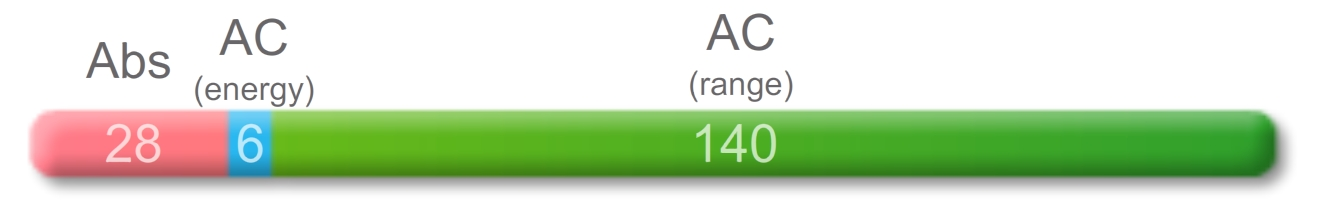
\includegraphics[scale=0.8]{figs_temp/features.jpg}
	\caption{Origin of the 174 features in features in feature configuration 2.}
	\label{fig:feat_fig}
\end{figure}

We can also choose to look at the Fourier transform, as in configuration 3. Using the \gls{dft} we reach a similar accuracy as in configuration 2 but require some 700 features. The 700 features are a result of computing a discrete Fourier transform along the slow time of all 28 ranges over 25 samples\footnote{Ideally, the \gls{dft} should be computed as an FFT over a number of slow time samples which is a power of 2. However, to get a fair comparison of the feature extraction methods, we utilize the same number of samples for all methods.}. The length of each transform is 25, and by concatenating them all into one feature vector, we end up with $28\cdot 25=700$ elements. 

The high accuracy and low number of features of configuration 2 makes it the clear top performer of the three, and will be used for the remainder of this report for further investigation.

\section{Feature Principal Component Analysis}

Through the feature extraction methods described in previous sections we obtain high dimensional feature vectors. Getting an intuitive feel for such high-dimensional data is difficult as direct plotting is limited to three dimensions. 

Principal component analysis (\gls{pca}) is  a classical technique in statistical data analysis which takes a large set variables from a multivariate dataset and finds a smaller set of variables with less redundancy. Critically, \gls{pca} finds a rotated orthogonal coordinate system such that the elements of the set become uncorrelated \citep{hyvasrinen_karhunen_oja_2004}. By projecting elements onto the principal axes corresponding onto the directions of maximal variance we obtain a good approximation of the original data in a lower dimension.

After having chosen to proceed with feature configuration 2 in table \ref{tab:feat}, the 174 dimensions can be reduced to 2 dimensions using \gls{pca}. By projecting feature vectors onto the two directions of maximal variance, we get a good visualization of the separability of the different surfaces as seen in figure \ref{fig:pca}. Note that each dot in this plot corresponds to one feature vector, and that the figure represents features extracted from the full set of 175 minutes of data sampled at 200 Hz.  

\begin{figure}[h]
	\centering
	\includegraphics[scale=0.50]{figs_temp/pca_analysis.png}
	\caption{By performing a principal component analysis on the feature vectors we project 174 dimensional feature vectors onto two dimensions corresponding to directions of maximum variance. This allows for us to visualize how separable the different surface types are.}
	\label{fig:pca}
\end{figure}



% Classification schemes
\chapter{Classification schemes}

In this chapter a few classification models are evaluated for the feature extraction processes described in the preceding chapter. Detailed descriptions of each classification framework is omitted, but good sources for further explanation will be supplied for the interested reader. The aim of this chapter is to compare various models and to determine the most promising one with regards to accuracy, size and complexity. 

\section{Evaluated models}

In this section the effectiveness of a few different models are compared. Two linear models and two non-linear models are evaluated. The two linear models considered, a \emph{Linear Discriminant Analysis} (LDA) and a \emph{Support Vector Machine} (SVM) model.

\subsection{Deep neural networks}

Deep neural networks, or DNN for short, are neural networks that has more than one layer of hidden units between its inputs and outputs \citep{hinton_deng_yu_dahl_mohamed_jaitly_senior_vanhoucke_nguyen_sainath_2012}. 


DNN's in various forms have gained immense popularity over the past two decades achieving considerable success within a wide spectrum of applications, such as in image recognition \citep{szegedy_liu_jia_sermanet_reed_anguelov_erhan_vanhoucke_rabinovich_2018}, acoustic modeling of speech \citep{hinton_deng_yu_dahl_mohamed_jaitly_senior_vanhoucke_nguyen_sainath_2012}, 

\subsection{LSTM}
Mention CNN and LSTM being used for time series classification. Then bring up the article which combines these two to motivate this approach.

Observing one range bin at a time, one could think of the radar data as a time series. This motivates the use of some classification scheme that exploits temporal behaviour. Recurrent neral networks (RNNs) feature this by having feedback within individual layers in the network. \citep{karim_majumdar_darabi_chen_2018} The problem with RNNs, however, is that they suffer from a vanishing or exploding gradient, and can only sustain a short term memory. A way to combat this is to use a neural network layer called long short term memory (LSTM). These are thoroughly described in, for example \citep{hochreiter_schmidhuber_1997}

LSTM-layers have previously been used successfully for classifications in radar applications. For instance in \citep{jithesh_sagayaraj_srinivasa_2018} the method was able to classify flying objects from $\textbf{nnn}$ different classes with an accuracy of ...? In \citep{karim_majumdar_darabi_chen_2018}, the LSTM layer is used in combination with a fully convolutional neural network (FCN), which proves to be a significant improvement from just using FCNs when classifying time series.

% Define block styles
\tikzstyle{decision} = [diamond, draw, fill=blue!20, 
    text width=4.5em, text badly centered, node distance=1.5cm, inner sep=0pt]
\tikzstyle{block} = [rectangle, draw, fill=blue!20, 
    text width=7em, text centered, rounded corners, minimum height=4em]
\tikzstyle{line} = [draw, -latex']
\tikzstyle{cloud} = [draw, ellipse,fill=red!20, node distance=3cm,
    minimum height=2em]
   

\begin{tikzpicture}[node distance = 3cm, auto]
	% Place nodes
	\node [block] (obtained) {Obtained data};
	\node [block, below left of=obtained] (training) {Training data};
	\node [block, below right of=obtained] (test) {Test data};
	\node [block, below of=training] (train pre) {Preprocess and extract features};
	\node [block, below of=test] (test pre) {Preprocess and extract features};
	\node [block, below right of=train pre] (est) {Estimate $\mathbf{\mu}_f$, $\mathbf{\sigma}_f$};
	\node [block, below left of=est] (scale train) {Scale to ZMUV};
	\node [block, below right of=est] (scale test) {Scale to ZMUV};
	\node [block, below of=scale train] (train model) {Train model};
	\node [block, below right of=train model] (Classify) {Classify};
	% Draw lines
	\path [line] (obtained) -| (training);
	\path [line] (obtained) -| (test);
	\path [line] (training) -- (train pre);
	\path [line] (test) -- (test pre);
	\path [line, dashed] (train pre) -| (est);
	\path [line,dashed] (est) -- (scale train);
	\path [line,dashed] (est) -- (scale test);
	\path [line] (test pre) -- (scale test);
	\path [line] (train pre) -- (scale train);
\end{tikzpicture}


% Postprocessing and optimization
\chapter{Postprocessing and optimization}

In the previous chapter a simple feed-forward neural network was found to be a suitable model for the surface classification problem investigated. In this chapter, some improvements and additions to this model are introduced. First, we perform some data augmentation to increase the number of training data. Then, removal of outliers using the clustering method DBSCAN is tested to see if accuracy can be further improved. Finally, two detection methods are discussed for outlier suppression.


\section{Data augmentation}

A recurring problem in training ANN's is that there simply isn't enough data \citep{lemley_bazrafkan_corcoran_2017}. Too little data will make a network prone to overfitting, which means that it becomes highly biased to what it has seen in training, and will subsequently perform poorly on any validation or test set. In the preceding chapter dropout was introduced for this particular purpose, and examining the cross validation accuracies it is clear that reasonable accuracy is attained without any further means.

However, by \emph{augmenting} the data we may be able to further increase the training set size, and subsequently further increase model performance. Data augmentation is the process of supplementing a dataset with similar data created from the same dataset. How one augments a dataset is data dependent. In for instance computer vision, data augmentation often involves rotating, translating, blurring or in some other way modifying existing images \citep{lemley_bazrafkan_corcoran_2017}.

In the present case of increasing the number of data batches from a given data square, we can allow for overlapping batches. Previously, when batches of length $T$ were generated from $Q$ slow time samples, every $T$ sweeps produced one batch providing a total of $Q/T$ batches for analysis. However, noting that any slow-time sequence of $T$ sweeps is a valid data batch, we may form overlapping batches from every $T/A$ samples, where $A$ is some integer factor selected so that $T/A$ becomes an integer. This produces $(A-1)(Q/T-1)$ additional batches providing a total $P$ batches of

\begin{equation}
	P = 
	\frac{Q}{T} + (A-1)\Big(\frac{Q}{T} - 1\Big) = 
	\frac{AQ}{T}-A+1.
\end{equation}


Setting $A=5$, one data rectangle consisting of 50,000 slow time samples normally yielding 2,000 data batches using $T=25$, instead produces 9996 data batches. Thus, with this method we are able to increase the number of training samples by almost a factor of 5. In table \ref{tab:aug}, the effects of data augmentation with $A=5$ is compared to having no augmentation.

% Discuss this result later on.

\begin{table}
	\label{tab:aug}
	\begin{center}
		\rowcolors{2}{gray!25}{white}
		\begin{tabular}{|c|c|}
			\hline
			\rowcolor{gray!150}
			\color{white}\textbf{Augmentation} & \color{white}\textbf{LOO Acc.} \\
			1 & 98.49 \\
			5 & 98.53 \\
			\hline
		\end{tabular}
	\end{center}
	\caption{Leave-one-out accuracies with and without data augmentation.}
\end{table}

%\section{Outlier removal}

%In any dataset some data corruption is to be expected. A grassy surface may have small patches of soil without grass, the device may have been moving at either a too high or too low velocity for a short period of time or the radar sensor iteslf may have had temporary issues. Such processes forms data points inconsistent with the overwhelming bulk of data, or \emph{outliers}, which negatively impacts model performance. The importance of outliers is dependant both of their frequency and magnitude, and can be significantly detrimental to model accuracy making effective removal of them often necessary or at least benifitial \citep{osborne_overbay_2004}, \citep{hodge_austin_2004}. 

\section{Detection of surface change}

Even with an optimized model with tons of training data, erronous predictions are unavoidable in any real-world scenario. Prediction probabilities are produced by the model rapidly, 8 times a second for a sampling rate of 200 Hz and a batch size $T=25$ according to equation \ref{eq:classification_rate}. With such errors present in the prediction confidences of the model, what is a reasonable strategy to detect when a change in surface has occurred?  

Many elaborate statistically appealing methods for change detection are presented in \citep{basseville_nikiforov_1993}. These methods require some basic assumptions on the data it attempts to detect a change from, such as for the data having constant probability distribution before and after a parameter change occurs. This, however, renders these methods difficult to use in the present use case, as we are dealing with the output of a highly nonlinear artificial neural network producing predictions with unknown structure. This is reinforced by examining what the model outputs, see the top figure in \ref{fig:trans_tgtg}. Predictions remain extremely stable for long periods of time, with occasional outlying predictions every now and then. These outlying predictions need be suppressed for stable change detection.

The perhaps most effective way of suppressing data littered with outliers is through some form of median filtering \citep{yin_yang_gabbouj_neuvo_1996}. Median filters is very robust against impulsive-type noise, a property that cannot be achieved by traditional linear filtering techniques. The regular form of a median filter simply takes the median of current and previous datapoints, resulting in an output significantly less sensitive to inconsistencies \citep{pearson_2002}. For a sequence $\{p\}$ of predictions, we apply a median filter of length $L$, and set a decision threshold $\xi$ to produce binary predictions $P_i$ according to
\citep{yin_yang_gabbouj_neuvo_1996}

\begin{equation}
	P_i=0 \quad\text{if}\quad\text{median}\{p\}_{i-L+1}^i\leq\xi, 
	\quad \text{else} \quad P_i = 1
\end{equation}

where $0<\xi<1$. The drawback of using median filtering is that a change is delayed a few predictions. Thus, th length $L$ must be selected so that the device has not moved too far before the change detection has occurred, but is still capable of sufficiently  suppressing outlying predictions. 


\iffalse
\section{Postprocessing and detection}


\begin{figure}
	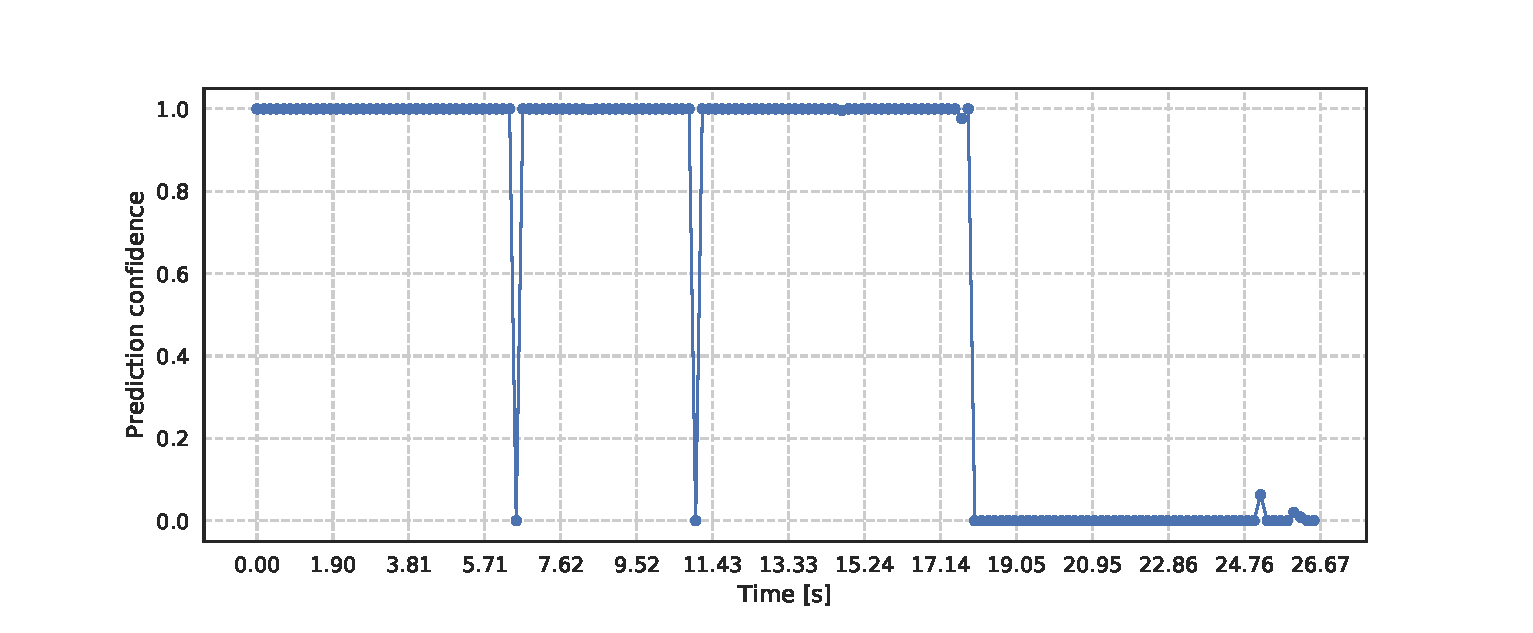
\includegraphics[scale=0.5]{figs_temp/detect_nothing}
	\label{fig:detect_no}
	\caption{Transition region with some outliers}
\end{figure}

\subsection{Thresholding}

The simplest possible detection algorithm is by setting a threshold $\xi$, and classifying below surface as either grass or non-grass depending on whether the prediction is above or below the set threshold. Denoting the resulting prediction as $P$ this detection algorithm is 

\begin{equation}
	P_i=0 \quad\text{if}\quad p_i\leq\xi, \quad
	\text{else} \quad P_i=1
\end{equation}

However, for this method to fail only a single incorrect prediction $p_i$ is required so the algorithm is extremely sensitive to any errors in $p$.

\begin{figure}
	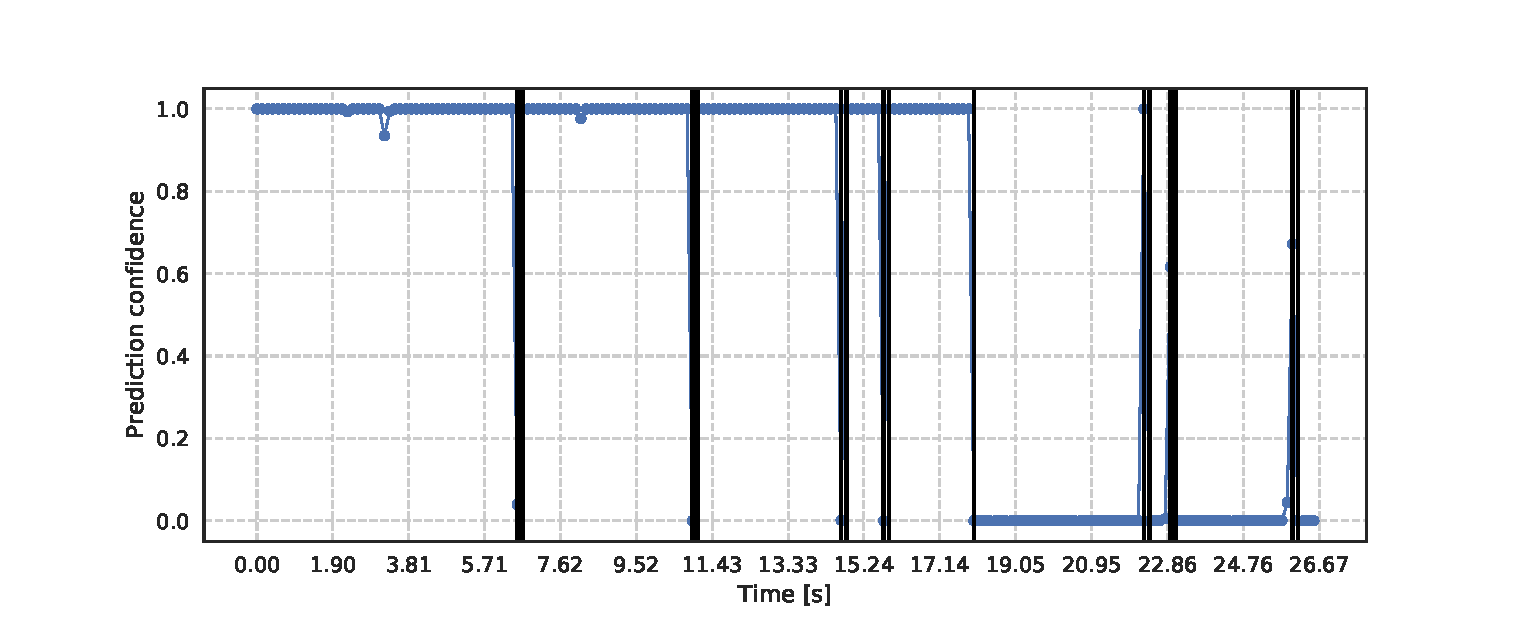
\includegraphics[scale=0.5]{figs_temp/detect_thresh}
	\label{fig:detect_thresh}
	\caption{Detecting transition region using thresholding.}
\end{figure}

\begin{figure}
	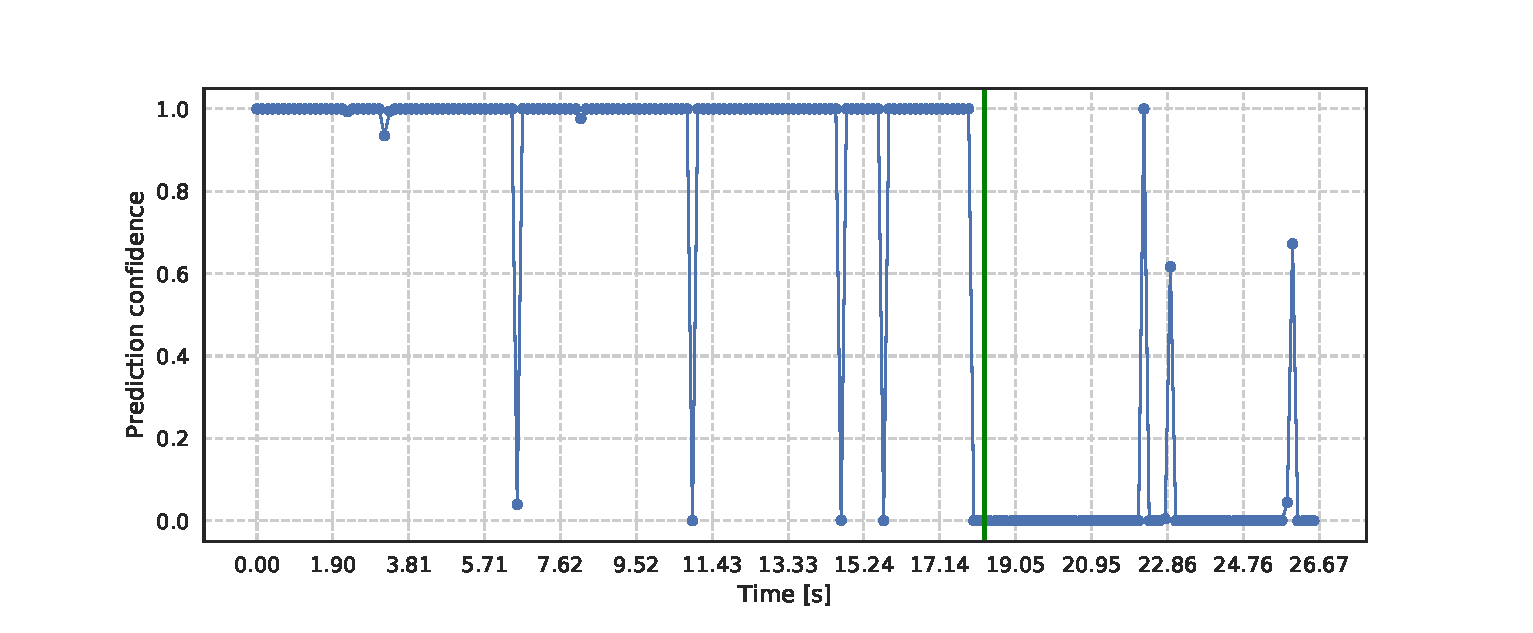
\includegraphics[scale=0.5]{figs_temp/detect_median}
	\label{fig:detect_median}
	\caption{Detection transition using median filtering}
\end{figure}

\subsection{CUSUM}

A traditional and statistically appealing method for effectively detecting abrupt changes in data is CUmulative SUM, hereby refered to as CUSUM. The cumulative sum computed in CUSUM is a log-likelihood $S$ defined through

\begin{equation}
	S_j^k = \sum_{i=j}^k \text{ln}\frac{p_{\theta_1}(y_i)}{p_{\theta_0}(y_i)}
\end{equation}

\begin{figure}
	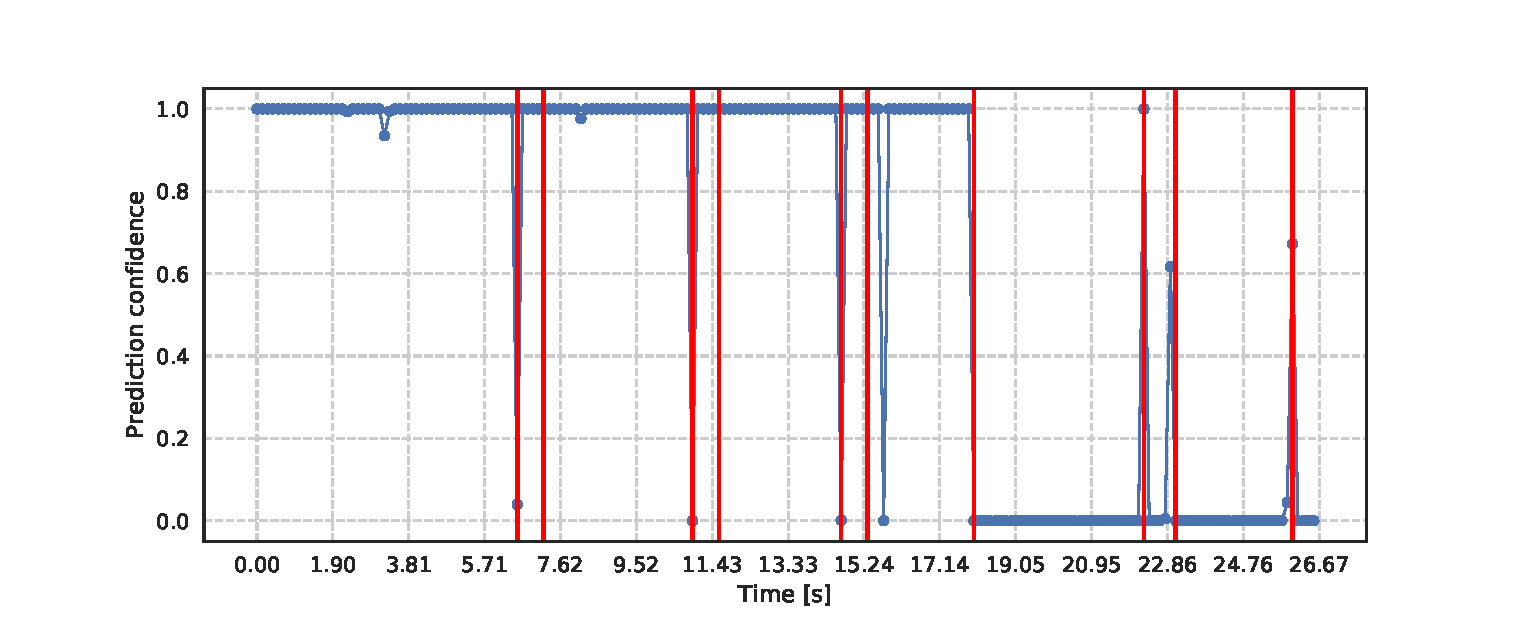
\includegraphics[scale=0.5]{figs_temp/detect_cusum}
	\label{fig:detect_cusum}
	\caption{Detection of transition using CUSUM.}
\end{figure}

[Continue explanation]






\subsection{Method comparison}

After introducing each detection algorithm a comparison is in order. Below is output from a typical transition using [model we made]. Each algorithm has been applied to the data for change detection.


Informal definition as data points inconsistent with our expectations

\section{Removal of outliers}


\subsection{Mahalanobis distance}

\subsection{DBSCAN}

\section{Hyperparameter optimization}
\fi




% Discussion
\chapter{Results and Discussion}
In this section the final model's capabilities are tested and discussed. Previously, the model has been evaluated on labeled data, thus generating a success rate. Below, the model will instead make predictions on unlabeled data, and instead output a confidence in its prediction.

Later on various things about the work are brought up for discussion.

\section{Real and artificial transition regions}

While we up to this point maily have focused on leave-one-out and validation set accuracies we have not in detail studied what the classifier output looks like. We are specifically interested in examining how well performance is when the robot moves across a \emph{transition region}, a region where the surface type changes from grass to nongrass or vice versa. Ideally the prediction should rapidly change according to the new target surface. 

This can be accomplished in two different ways. The first revolves around creating a test set by concatenating the last parts of each session. By doing this, we artificially generate transition region data which we can predict on. Examining these predictions we get a feel for what output the predictor may generate when moving from one surface to the next. The second method is to simply use real-world measurements from when the robot moves across a surface. We should see that at the time point when the robot has reached the transition the prediction change accordingly. 

In the first test, four surfaces are concatenated into a sequence: grass, asphalt, grass, tiles. The predictions are shown in the top part of figure \ref{fig:artificial1}. Below, the predictions are median filtered with filter length $L=5$, see section \ref{surface_change}. The outliers are removed, rendering a very accurate description of the scene. 

Two more challenging surfaces according to table \ref{tab:loo} are soil and gravel. In figure \ref{fig:artificial2} the predictions on artificial transitions including these are displayed. With median filtering we obtain equally good results. Something worth noting in the two figure is that the surface transition is delayed by two steps after the median filtering. It is important to be aware of what distance this corresponds to in the physical world, since we do not want to detect an edge long after it is passed. Each prediction uses 25 samples, and with a delay of two predictions this means a 50 sample delay. With a sample frequency of 200 Hz, this means a 0.25 second delay in the edge detection, or traveling at the speed $v=0.3$ m/s, a delay corresponding to $0.3\cdot0.25=0.075$ m.

Looking at the high leave-one-out accuracies in table \ref{tab:loo}, the results of classifications upon the artificial transitions may not come as a surprise, as they are based on the same data. What we can see here, however, is that not only does the model classify correctly, but it does so with a very high confidence. To test the model even further, it will make predictions of real world transitions, not included in our dataset. Figure \ref{fig:trans_tgtg} shows a transition from grass to tiles, and figure \ref{fig:trans_gg} a transition from grass to gravel. Focusing on the median filtered predictions, we see that outside the transition region, the model works well for classifying both materials. What happens around the transition is perhaps more interesting. In the previous figures, the predictions went from 1 to 0 and vice versa in just one step. Here, it takes a while before the model reaches zero-outputs. There are two possible explanations for this. First of all, in the artificial transitions, the surface went from a perfect grass surface to a perfect non-grass surface at an instance. In real transitions, there might be some overlap of grass on the non-grass surface, making the model unsure of what it sees. Another explanation could be that one sensor is facing straight down, whereas the other one looks slightly more forward. Hence, the model is perceiving both grass and tiles simultaneously during a short time. 

The results show great promise, but the work is still at an early stage. The surfaces in the four transitions were intentionally free from as many obstructions as possible. When facing surfaces with characteristics not taken into regard by the model, the results will not likely be as good. 

\begin{figure}
	\centering
	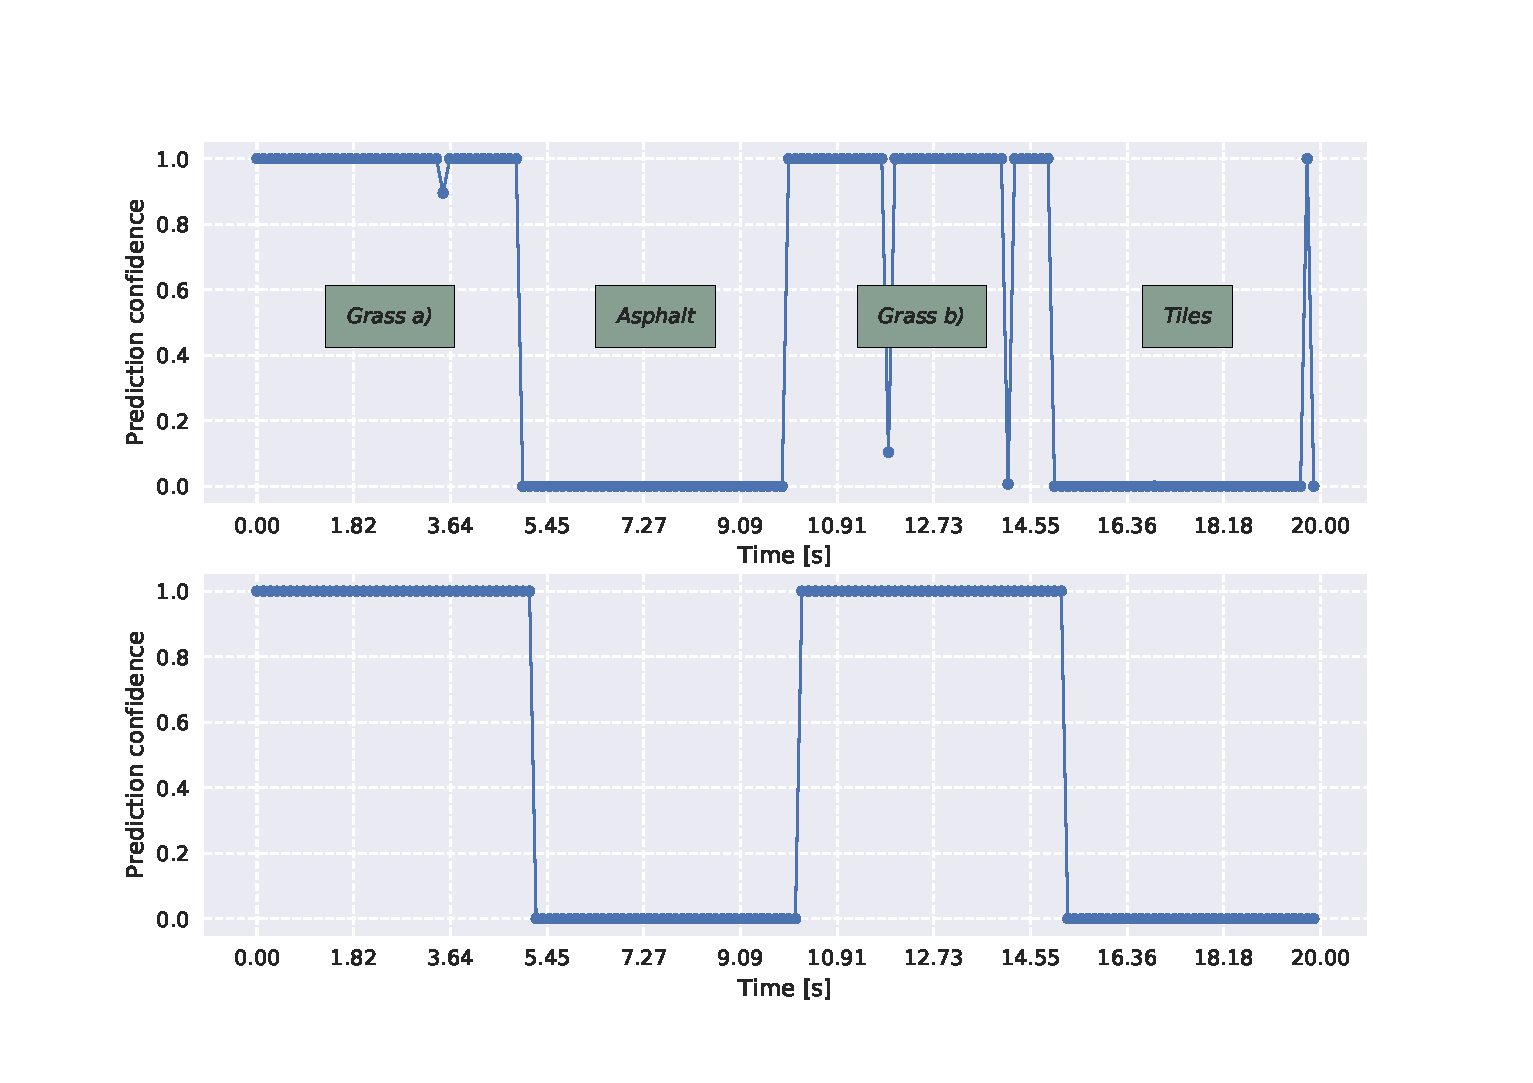
\includegraphics[scale=0.5]{figs_temp/varmats1}
	\caption{Predictions on an artificial transition region created using samples from four different regions. The bottom figure shows the median filtered predictions with filter length $L=5$.}
	\label{fig:artificial1}
\end{figure}

\begin{figure}
	\centering
	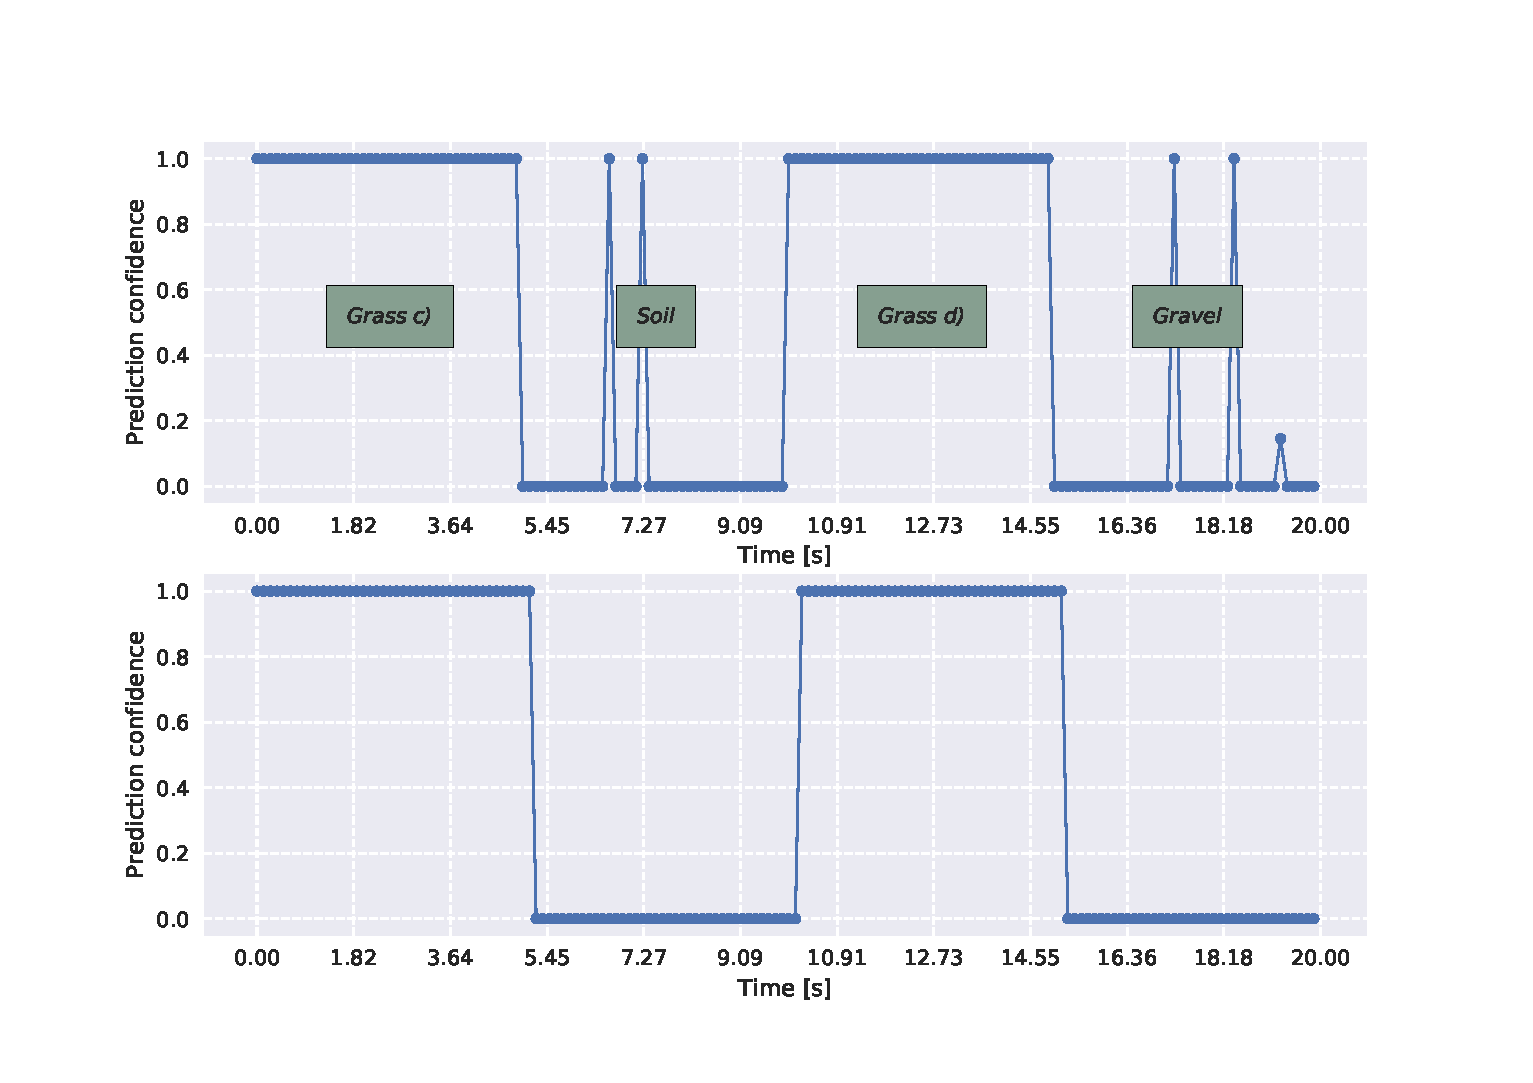
\includegraphics[scale=0.5]{figs_temp/varmats2}
	\caption{Predictions on an artificial transition region created using samples from four different regions.}
	\label{fig:artificial2}
\end{figure}

\begin{figure}
	\centering
	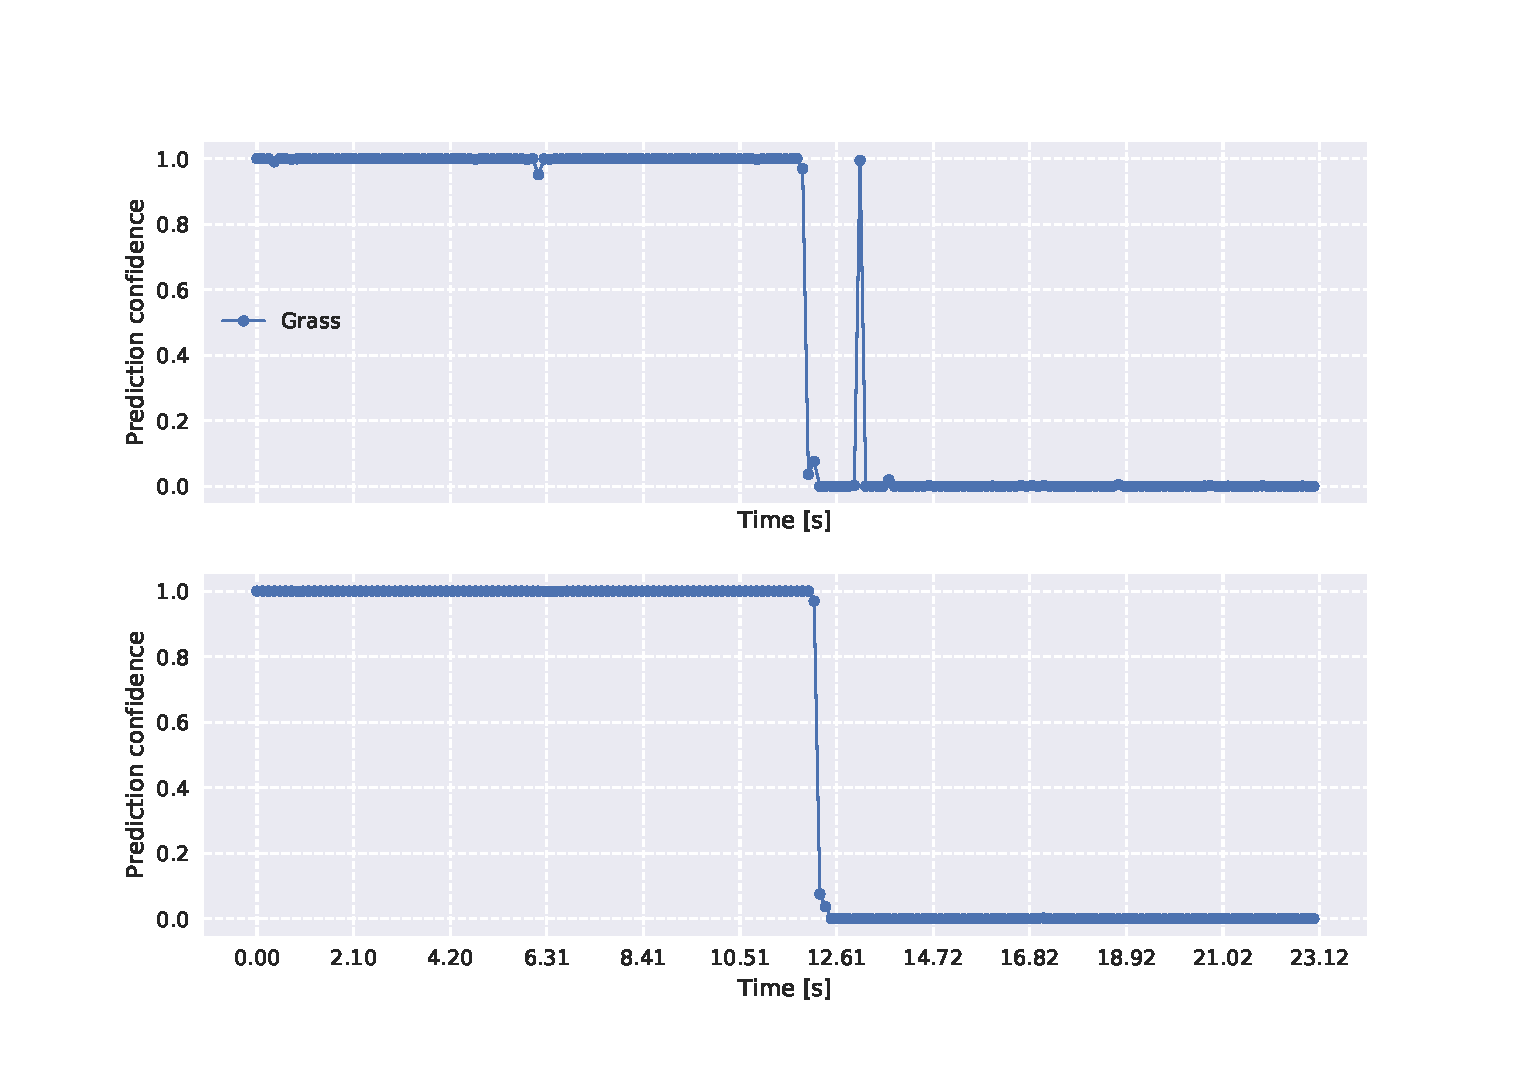
\includegraphics[scale=0.5]{figs_temp/transition_grass_tiles_grass}
	\caption{Predictions from a real-world test where the robot moved from grass to a tiled pavement.} 
	\label{fig:trans_tgtg}
\end{figure}

\begin{figure}
	\centering
	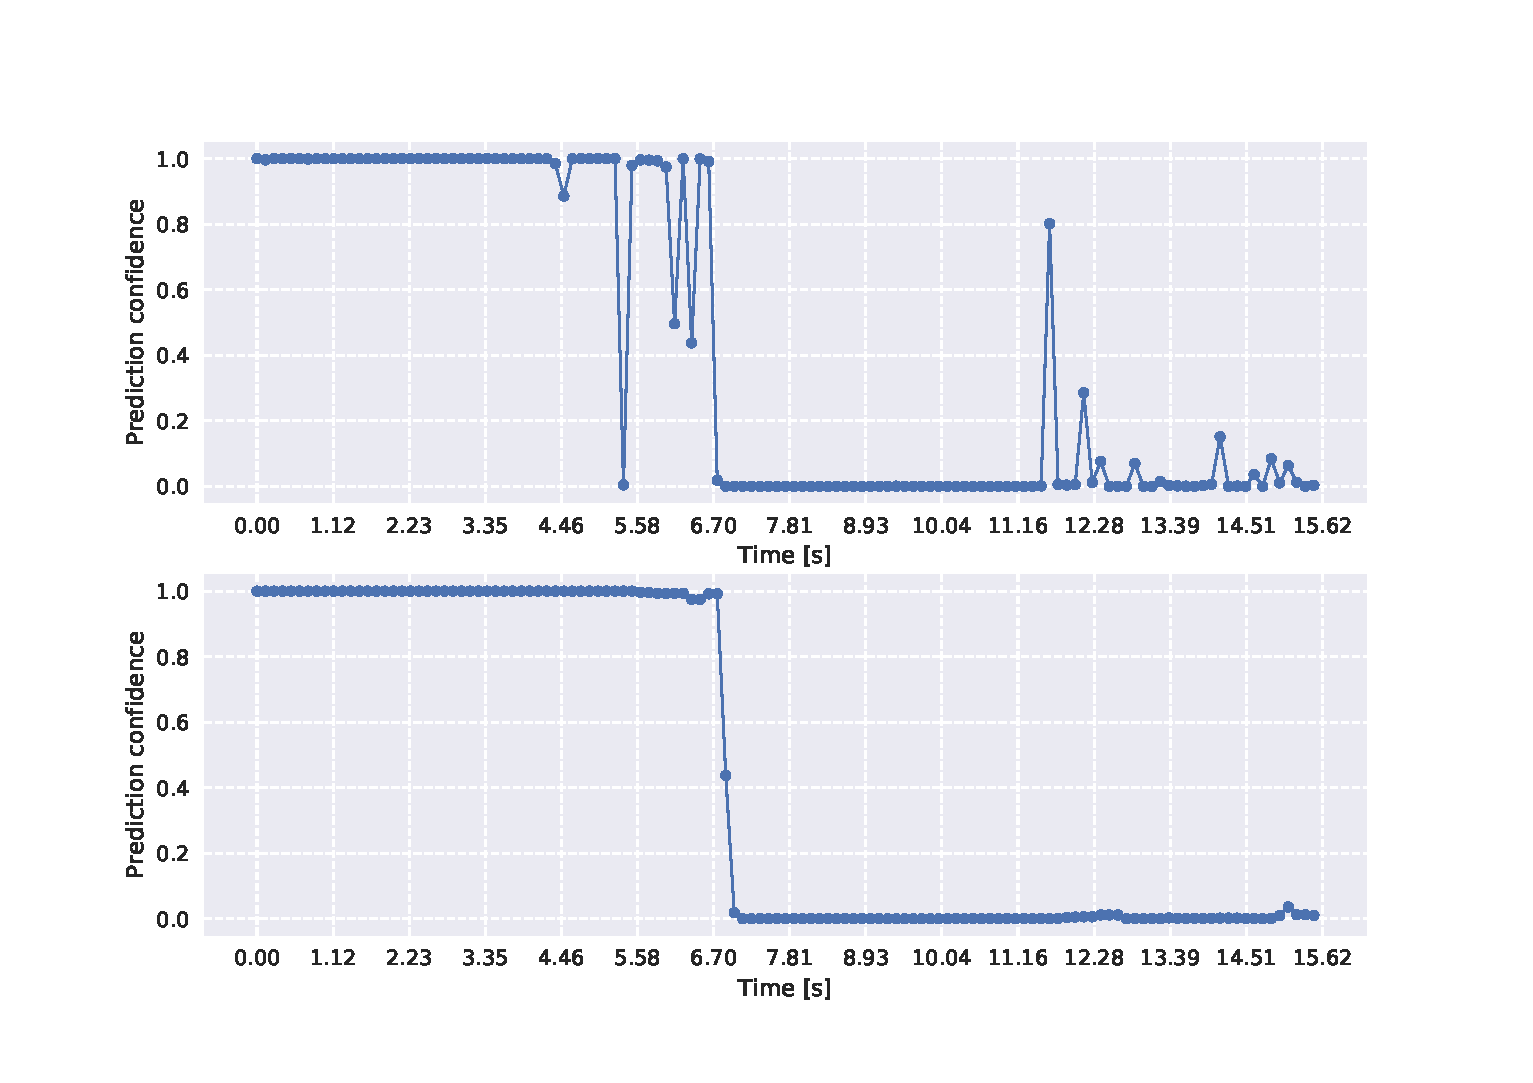
\includegraphics[scale=0.5]{figs_temp/transition_grass_gravel2}
	\caption{Predictions from a real-world test where the robot moved from grass to gravel.}
	\label{fig:trans_gg}
\end{figure}

\section{Difficult surfaces}
While we only have five material classes in this work, each class can be broken down to multiple subclasses. Taking grass as an example, it may vary in a wide range of attributes such as length, humidity and sparsity to name a few. Therefore it is important to gather a dataset as diverse as possible, so that the model has trained on all common varieties of each surface. 

However, the model can only be prepared for so much, and an often critical aspect of any machine learning system is its performance on dissimilar data. It is difficult to foresee how a complex neural network will interpret a surface displaying characteristics not included in training. For instance, what would the model make of a lawn which is partially covered by leaves and twigs; or a surface type it has never seen before? Perfecting the model to work in any surrounding calls for a good sense of what difficulties may occur, as well as a large time investment. 

%\section{Moisture}

%One particularly challenging aspect of adequately classifying surfaces is the ever-changing environmental conditions surronding the sensor. Of particular interest is the moisture content in the surfaces of interest. Greater soil moisture implies higher dielectric constant, which in turn increases radar wave scattering \citep{rappaport_2006}. Thus a single surface may very well change its scattering properties over time. 

% More things that make selecting data tricky

%\section{Surface variances}


%Such effects is difficult to account for when selecting data. Gather a dataset as diverse as possible



\section{Feature Extraction and Model Selection}
\label{disc_feat}
Table \ref{tab:loo} is in many ways a very telling one. Here, each sample session was classified without using any of the samples from the session at hand. Instead, all other sessions were used in training. Six different methods of classification were evaluated; two linear and four nonlinear. 

First and foremost it is noted that each tested method performed at the very least \emph{decently}. One may argue that the \gls{lstm} model is unstable or that using \gls{lda} produces lower accuracy predictions, but they nonetheless generated accuracies above 97\% on average. Considering these are the lower-performing classifiers, and the remaining ones perform even better, suggests that the performed feature extraction captures, or at least maintains, the cruicial information in the original data. 

Some may argue that no feature extraction should be performed when working with deep neural networks; that the networks are complex enough to find good features on their own. If this is true, the network may yield a better result by omitting the feature extraction as this could discard information in the original data. However, since much of the informations seems to be found in how signals evolve over time, a network with no feature extraction would require multiple sweeps to be concatenated into one feature vector in order to be able to find these time dependencies. Say it would take 25 (downsampled) sweeps, each with 14 range bins. Each sweep would then produce 28 features as the real and imaginary part are divided into separate features. The feature vector to such a network would then consist of $25\cdot 28=700$ features. While this could \textit{potentially} slightly increase the already great accuracies, the feature extraction reduces the number of features (and thereby computational cost) and - if done properly - represents samples with more robust features that are material specific.

On a different note, the final choice of classifier is also debatable. The \gls{dnn} classifier was chosen mainly because of its high leave-one-out scores in table \ref{tab:loo}. But without blindly chasing an accuracy as high as possible, the results of the linear models are good enough to suggest that the data could be at least \textit{approximately} linearly separable. If it were, a non-linear model would not be necessary, hence further investigation in linear models is motivated.

\section{Errors and Uncertainties}
As with all works, there are things that can go wrong due to either technical reasons or human reliability. The data collecting process is a prime example of where human reliability is inevitable. Here, fundamental decisions are made, which the entire work is based upon. For instance, in general, one strives for a dataset where the numbers of samples from each class are as balanced as possible. But the question of what a balanced dataset \textit{is}, sometimes holds multiple answers. In this work, there are four different types of materials belonging to class 0 (not grass) and one belonging to class 1. A natural question to ask oneself is whether there should be equally many samples for each \textit{material}, or equally many for each \textit{class}. We have chosen to balance the dataset so that there are approximately as many samples in each class. If all grass surfaces looked the same, this would perhaps make the model biased in its predictions, but due to the great variety among grass surfaces the bias is eliminated.

Another risk when collecting data is obtaining too little of it. However, looking at how high accuracies the models achieve as well as how little improvement the data augmentation yields, it is not likely that we provide too little data to our models.

A more technical uncertainty regards the assumption of a constant velocity. When facing a rough terrain or steep hills, the robot's velocity is bound to change. As both the \gls{dft} and autocovariance require a consistency in the spacing between sample points, we cannot tolerate too large variations in velocity. Hence, to sample at regular distaces the sampling could be controlled by positional feedback from the robot rather than a fixed sampling frequency.

While this work has not put much focus on \textit{live} classifications, this does pose a new limitation on the model. Ideally we want the system to collect $T$ samples, and make an instantaneous prediction so that $T$ new samples can be collected right away. By running the system on a single thread, however, the time it takes to generate a prediction delays the data collecting process with some time $t_{cl}$, as only one process can be ran at a time. An alternative could be to handle the classifications in a separate thread. That way, data could be collected continously, while classifications are performed in parallel. Doing this requires caution. If the time it takes to generate a classification exceeds the time it takes to collect $T$ samples, i.e. $t_{cl}>T/F_s$, a delay will accumulate over time. After a while predictions would be irrelevant as they would be based on surfaces far behind the robot. A natural limitation to assign the model is therefore
\begin{equation}
	t_{cl} \le \frac{T}{F_s}.
\end{equation}
The time $t_{cl}$ has not been discussed in this work, but is highly relevant to study in the future.



% This remarkable result means that given a random sample from the dataset collected, with no samples from the session the sample was taken from used in training, we can correcly classify the surface as grass or non-grass 39/40 times even with the lower-performing classifiers. With the top performing fully connected model, even higher accuracy was obtained with a low standard deviation. 




\bibliography{refs}
\bibliographystyle{apalike}

% Appendices


\begin{appendices}

	\chapter{IQ Demodulation}
	IQ demodulation is a major part in the receiver processing of radar data. After going through the mixing process, the signal can be expressed as \citep{lee_1991}
\begin{equation}
\label{eq:signal}
	x_R(t)=A(t)\sin(\Omega t+\theta(t)).
\end{equation}
Here, $\Omega$ is the carrier frequency of the transmitted pulse and the time, $t$, relates to distance according to equation \textbf{*ref*}. The goal of IQ demodulation is to extract $A(t)$ and $\theta(t)$ from \eqref{eq:signal}, and end up with a complex signal of the form $A(t)e^{i\theta(t)}$.

Most classical radars follow the demodulation scheme depicted in figure *ref*. The first step is to split the signal in \eqref{eq:signal} into two separate channels. In the upper channel, the signal is multiplied by a sinusoid which is generated with the same carrier frequency as the received pulse. The result of this multiplication can be rewritten as
\begin{gather}
	 A(t)\sin(\Omega t+\theta(t))\cdot 2\sin(\Omega t) = \\
	\label{eq:split}
 	 A(t)\cos(\theta(t))-A(t)\cos(2\Omega t+\theta(t)).
\end{gather}
The next step in the demodulation scheme is to low pass filter the signal. Thus, the high frequency term in \eqref{eq:split} is removed, and only $A(t)\cos(\theta(t))$ remains. We define this as $I(t)$.

Similarly, in the bottom channel in figure *ref to schematics*, the original signal is multiplied by a generated wave signal of the same carrier frequency. However, this time, the signal is shifted 90 degrees in phase. Just as before, we may rewrite the product as
\begin{gather}
	 A(t)\sin(\Omega t+\theta(t))\cdot 2\cos(\Omega t) = \\
	\label{eq:split2}
 	 A(t)\sin(\theta(t))+A(t)\sin(2\Omega t+\theta(t)).
\end{gather}
After low pass filtering we obtain $A(t)\sin(\theta(t))$, which we define as $Q(t)$. Finally, by defining $I$ and $Q$ as the real- and imaginary parts of a complex number, respectively, we have our IQ-data
\begin{equation}
	I(t)+iQ(t)=A(t)\Big(\cos(\theta(t))+i\sin(\theta(t))\Big)=A(t)e^{i\theta(t)}
\end{equation}

\end{appendices}

\end{document}
